%
% Elliott Hudson College - Maths Booklet Template
% Originally created on: May 3rd 2021
%
% Copyright (C) 2021 Ellis Dickinson
%
% LICENSE:
% This program is free software: you can redistribute it and/or modify
% it under the terms of the GNU General Public License as published by
% the Free Software Foundation, either version 3 of the License, or
% any later version.
%
% This program is distributed in the hope that it will be useful,
% but WITHOUT ANY WARRANTY; without even the implied warranty of
% MERCHANTABILITY or FITNESS FOR A PARTICULAR PURPOSE.  See the
% GNU General Public License for more details.
%
% You should have received a copy of the GNU General Public License
% along with this program. If not, see <https://www.gnu.org/licenses/>.
%
%
% IMPORTANT!!!!
% When compiling this document, please use XeLaTeX
% Other compilers do not support some of the features within this document.
%
\documentclass[fleqn]{article}

\setcounter{section}{6}                                          % Set the Unit Number (without Leading 0's)
\newcommand{\coursetitle}{A-Level Further Mathematics}           % Set the Course Title
\newcommand{\bookletunittitle}{Chi-Squared Tests}                % Set the Unit Title
\newcommand{\bookletsubtitle}{Content last revised by: S Waugh}  % Set the Subtitle
\newcommand{\unitprefix}{FS}                                     % Set the Unit Prefix

% DO NOT MODIFY THIS FIILE
% ----------------------------------------------
\usepackage[dvipsnames]{xcolor}
\usepackage[a4paper, portrait, margin=1.9cm]{geometry}
\usepackage{titlesec}
\usepackage{tikz}\usetikzlibrary{shapes.misc}\usetikzlibrary{calc}
\usepackage{setspace}
\usepackage{fontspec}
\usepackage[most]{tcolorbox}
\usepackage{varwidth}
\usepackage[inline]{enumitem}
\usepackage{multicol}
\usepackage{fancyhdr}
\usepackage{booktabs, tabularx}
\usepackage{mathtools}
\usepackage{tasks}
\usepackage{anyfontsize}
\usepackage[export]{adjustbox}		% http://ctan.org/pkg/adjustbox




\newcounter{taskscounter}
\settasks{							% Multi-column enumeration
	style=enumerate,
	counter=taskscounter,
	label-width={22pt},
	item-indent={15pt},
	label-align=right,
	label=\textbf{\alph*},
	before-skip = -\parskip , 		% undo paragraph skip
  	after-skip = -\parskip , 		% undo paragraph skip
  	after-item-skip = -\parskip+1mm	% undo paragraph skip
%   debug=true 						% useful for fine-tuning or debugging
}



% Define dynamic titlebars for sections/exercises
\newlength{\sectionnumberwidth}
\newcommand\titlebar{\hspace*{-0.1cm}
	\tikz[baseline, trim right=3.1cm] {
		\settowidth{\sectionnumberwidth}{
			\pgfinterruptpicture
				\textbf{\sffamily\thesection.\thesubsection}
			\endpgfinterruptpicture
		}
	    \fill [cyan!25, rounded corners=0.15cm] (2.5cm,-1.28ex) rectangle (\textwidth-\sectionnumberwidth+2.65cm,2.615ex);
	    \node [
	        fill=blue!60!white,
	        text=white,
	        anchor= base east,
	        rounded rectangle,
	        inner sep = 2mm,
	        minimum height=3.89ex] at (3cm,0) {
	        {\bfseries\thesection.\thesubsection}
	    };
	}
}
\newcommand\exercisebar{\hspace*{-0.1cm}
	\tikz[baseline, trim right=3.1cm] {
		\settowidth{\sectionnumberwidth}{
			\pgfinterruptpicture
				\textbf{\sffamily\thesection.\thesubsubsection}
			\endpgfinterruptpicture
		}
	    \fill [red!25, rounded corners=0.15cm] (2.5cm,-1.265ex) rectangle (\textwidth-\sectionnumberwidth+2.65cm,2.64ex);
	    \node [
	        fill=cherryred!80!white,
	        text=white,
	        anchor= base east,
	        rounded rectangle,
	        inner sep = 2mm,
	        minimum height=3.9ex] at (3cm,0) {
	        {\bfseries\thesection\thesubsubsection}
	    };
	}
}

\newtcolorbox{mybox2}[2][]{
	enhanced,
	before skip=2mm,after skip=2mm,
	colback=black!5,
	colframe=black!50,
	boxrule=0.2mm,
	attach boxed title to top left={
		xshift=1cm,yshift*=1mm-\tcboxedtitleheight},
		varwidth boxed title*=-3cm,
		boxed title style={frame code={
            \path[fill=tcbcolback!30!black]
              ([yshift=-1mm,xshift=-1mm]frame.north west)
                arc[start angle=0,end angle=180,radius=1mm]
              ([yshift=-1mm,xshift=1mm]frame.north east)
                arc[start angle=180,end angle=0,radius=1mm];
            \path[left color=tcbcolback!60!black,right color=tcbcolback!60!black,
              middle color=tcbcolback!80!black]
              ([xshift=-2mm]frame.north west) -- ([xshift=2mm]frame.north east)
              [rounded corners=1mm]-- ([xshift=1mm,yshift=-1mm]frame.north east)
              -- (frame.south east) -- (frame.south west)
              -- ([xshift=-1mm,yshift=-1mm]frame.north west)
              [sharp corners]-- cycle;
            },interior engine=empty,
          },
	fonttitle=\sffamily\bfseries,
    title={#2},
    before upper = \sffamily,
    #1
}
          
\tcbset{%
    example/.style={%
        enhanced,
        breakable,
        rounded corners,
        toprule=0pt, rightrule=0pt, bottomrule=0pt, leftrule=1mm,
        colback=#1!5, colframe=#1!80!black, coltitle=#1!80!black,
        fonttitle=\bfseries\large\sffamily,
        detach title,
        before upper={\tcbtitle\quad},
        fontupper=\linespread{1.2}\selectfont
    },
    note/.style={%
        enhanced,
        breakable,
        separator sign none,
        rounded corners,
        toprule=0pt, rightrule=0pt, bottomrule=0pt, leftrule=1mm,
        colback=#1!5, colframe=#1!80!black, coltitle=#1!80!black,
        fonttitle=\bfseries\large,
        detach title,
        before upper={\sffamily\tcbtitle\quad\hspace{-2mm}},
        fontupper=\linespread{1.2}\selectfont
    }
}
\newtcbtheorem[auto counter]{examplebox}{Example}
{example=blue}{ex}
\newtcbtheorem{practice}{Independent Practice}
{example=practiceorange}{pr}
\newtcbtheorem{note}{#1\hspace{-1mm}}
{note=notecolor}{nt}



% Custom Colour Definitions
\definecolor{practiceorange}{RGB}{252, 191, 0}
\definecolor{notecolor}{RGB}{0, 0, 0}
\definecolor{cherryred}{RGB}{191,0,0}

\definecolor{ehclogoblue}{RGB}{0,187,211}
\definecolor{ehclogogray}{RGB}{33, 34, 33}
\definecolor{ehclogoorange}{RGB}{243, 108, 33}
\definecolor{separatorgray}{RGB}{210, 210, 210}



\setstretch{1.1} 										% Globally adjust bullet spacing
\setlength{\parindent}{0cm} 								% Removes paragraph indent
\setlength{\multicolsep}{6.0pt plus 2.0pt minus 1.5pt}	% Halves whitespace before multicol environment
\setlength\tabcolsep{0pt} 								% Removes default space between columns in table

% Change various spacings of bulleted/numbered lists
\setlist[itemize]{topsep=2pt, itemsep=-2pt}
\setlist[enumerate]{topsep=-2pt, partopsep=4mm, itemsep=0pt}

% Change spacing of aligned mathematics
\AtBeginDocument{
	\setlength\abovedisplayskip{3pt}
	%\setlength{\belowdisplayskip}{0pt}
	\setlength\belowdisplayskip{7pt}
	%\setlength{\belowdisplayshortskip}{0pt}
}


\setsansfont{AptiferSansPro}[
	Path = fonts/,
	Extension = .ttf,
    UprightFont = *-Regular,
    BoldFont = *-Medium
]



% Implement the custom titlebars
\titleformat{\section}{\large\sffamily}{\titlebar}{0.1cm}{}
\titleformat{\subsection}{\large\sffamily}{\titlebar}{0.1cm}{}
\titleformat{\subsubsection}{\large\sffamily}{\exercisebar}{0.1cm}{}



% Define the easier get functions for sections and subsections
\renewcommand*{\thesection}{\arabic{section}}
\renewcommand*{\thesubsection}{\arabic{subsection}}
\renewcommand*{\thesubsubsection}{\Alph{subsubsection}}
\newcommand\getcurrentref[1]{%
 \ifnumequal{\value{#1}}{0}
  {??}
  {\the\value{#1}}%
}
\newcommand{\exercise}{\subsubsection}



%Custom font size 'YUGE', larger than huge
\newcommand\YUGE{\fontsize{35}{35}\selectfont}

% Define custom footer
\fancypagestyle{plain}{
	\fancyhf{} % clear all header and footer fields
	\fancyfoot[OC]{ %right hand side
		\vspace{-0.7em}
		\hfill {\sffamily\raggedright {\color{separatorgray}\getcurrentref{page}} \\}\vspace{-1.6em}
		\begin{minipage}{.3\linewidth}
			\color{separatorgray}\rule{\linewidth}{0.4pt}
		\end{minipage}
		\begin{minipage}{.1\linewidth}
			\centering
			
\includegraphics[scale=0.4]{images/ehc-brand-separator-icon}
		\end{minipage}
		\begin{minipage}{.3\linewidth}
			\color{separatorgray}\rule{\linewidth}{0.4pt}
		\end{minipage}
	}
	\fancyfoot[EC]{ %left hand side
		\vspace{-0.7em}
		{\sffamily\raggedright {\color{separatorgray}\getcurrentref{page}} \\}\vspace{-1.6em}
		\begin{minipage}{.3\linewidth}
			\color{separatorgray}\rule{\linewidth}{0.4pt}
		\end{minipage}
		\begin{minipage}{.1\linewidth}
			\centering
			
\includegraphics[scale=0.4]{images/ehc-brand-separator-icon}
		\end{minipage}
		\begin{minipage}{.3\linewidth}
			\color{separatorgray}\rule{\linewidth}{0.4pt}
		\end{minipage}
	}

	\renewcommand{\headrulewidth}{0pt}
	\renewcommand{\footrulewidth}{0pt}
}
\pagestyle{plain}



% Function for adding vspace above underbrace
\newcommand*\addunderbracespace[1]{\vrule width0pt height0pt depth#1\relax}


\newcommand{\formattedunittitle}{Unit P\getcurrentref{section}}

\bluetheme

% Preamble Overrides
\setlength{\tabcolsep}{1mm}

\hypersetup{
    % pdftoolbar=true,                      % Show Acrobat’s toolbar?
    % pdfmenubar=true,                      % Show Acrobat’s menu?
    % pdffitwindow=false,                   % Window fit to page when opened
    % pdfstartview={FitH},                  % Fits the width of the page to the window
    pdftitle={\bookletunittitle},           % Title
    pdfauthor={Stephen Waugh},              % Author
    pdfsubject={\coursetitle},              % Document Subject
    pdfcreator={Elliott Hudson College},    % Creator of the document
    pdfproducer={Elliott Hudson College}    % Producer of the document
}

% Document Content Starts Here
\begin{document}
% DO NOT MODIFY THIS FIILE
% ----------------------------------------------
% Title Page
% ----------------------------------------------
% Modified from a post from a post by ModyTex
% https://www.reddit.com/r/LaTeX/comments/faij1n/my_first_cover_page_done_in_latex_is_it/
% ----------------------------------------------
\pagestyle{empty}
\begin{tikzpicture}[overlay,remember picture]
    \begin{scope}[transform canvas ={rotate around ={45:($(current page.north)+(-1.5,-3)$)}}]
    \shade[rounded corners=12pt, left color=gray!80, right color=gray!80] ($(current page.north)+(-2,-6.7)$) rectangle ++(9,0.8);
    \end{scope}

    \begin{scope}[transform canvas ={rotate around ={45:($(current page.north)+(-3,-8)$)}}]
    \shade[rounded corners=20pt, left color=lightgray!80, right color=lightgray!80] ($(current page.north)+(2.5,-8)$) rectangle ++(15,1.35);
    \end{scope}

    \begin{scope}[transform canvas ={rotate around ={45:($(current page.north west)+(4,-15.5)$)}}]
    \shade[rounded corners=20pt, left color=ehclogoorange, right color=ehclogoorange] ($(current page.north west)+(15,-16)$) rectangle ++(20,1.5);
    \end{scope}

    \begin{scope}[transform canvas ={rotate around ={45:($(current page.north west)+(13,-10)$)}},]
    \shade[rounded corners=18pt, left color=ehclogoblue ,right color=ehclogoblue] ($(current page.north west)+(14.5,-10)$) rectangle ++(15,1.3);
    \end{scope}

    \begin{scope}[transform canvas ={rotate around ={45:($(current page.north west)+(18,-8)$)}},]
    \shade[rounded corners=8pt, left color=ehclogogray, right color=ehclogogray] ($(current page.north west)+(18.5,-8)$) rectangle ++(15,0.6);
    \end{scope}

    \begin{scope}[transform canvas ={rotate around ={45:($(current page.north west)+(19,-5.65)$)}},]
    \shade[rounded corners=12pt, left color=lightgray, right color=lightgray] ($(current page.north west)+(15.5,-5.65)$) rectangle ++(15,0.8);
    \end{scope}

    \begin{scope}[transform canvas ={rotate around ={45:($(current page.north west)+(20,-9)$)}}]
    \shade[rounded corners=15pt, left color=ehclogoorange, right color=ehclogoorange] ($(current page.north west)+(20,-8.4)$) rectangle ++(14,1.1);
    \end{scope}
\end{tikzpicture}

\vspace{-0.5cm}

\includegraphics{images/branding/brand-logo-vector}

\vspace{8.5cm}
\begin{minipage}{\textwidth}
    \sffamily

    \vspace{2mm}
    {\YUGE \raggedleft\bookletunittitle\\}

    \vspace{1mm}
    {\huge \raggedleft\coursetitle { }-- \formattedunittitle\\}

    \vspace{2mm}
    {\small \raggedleft\bookletsubtitle\\}
\end{minipage}
\vfill
% Key Information
% ----------------------------------------------

\begin{adjustbox}{valign=b}
	\begin{minipage}{.85\textwidth}
		\begin{mybox2}[colbacktitle=green]{Key Information}
			\textbf{Key Formulae:}
			\[
			\begin{aligned}
				x^a \times x^b &= x^{a+b} \\
				x^a \div x^b &= x^{a-b} \\
				(x^a)^b &= x^{ab} \\
				x^{-n} &= \dfrac{1}{x^n} \\
				x^{\tfrac{1}{n}} &= \sqrt[\textstyle{^n}]{x} \\
				a^2 - b^2 &= (a-b)(a+b)
			\end{aligned}
			\]

			\textbf{Key Terms:}
			\begin{itemize}
				\item \textbf{Expanding Brackets:} Multiplying brackets out
				\item \textbf{Factorising Brackets:} Putting expressions back into brackets
				\item \textbf{Surd:} A root of a number which can't be written as a whole number or fraction
				\item \textbf{Rationalising Denominator:} Removing the surd from the bottom of the fraction
			\end{itemize}
		\end{mybox2}
	\end{minipage}
\end{adjustbox}
\begin{minipage}[b]{.13\textwidth}
	\sffamily
	Solution Bank:
	\vspace{1mm}\linebreak
	
\includegraphics[scale=0.15, valign=b]{images/link-to-y1-sol-bank}
\end{minipage}


\begin{keyinformation}{images/links/f-maths/f-stats-1}
    \begin{enumerate}
        \item The \textbf{null} and \textbf{alternative hypotheses} generally take the following form:        \\
            H\textsubscript{0}: There is no difference between the observed and the theoretical distribution. \\
            H\textsubscript{1}: There is a difference between the observed and the theoretical distribution.
        \item \textbf{Goodness of fit} is concerned with measuring how well and observed frequency distribution fits to a known distribution.
        \item The measure of \textbf{goodness of fit} is $X^2={\mathlarger{\sum}} \dfrac{(O_i-E_i)^2}{E_i}$ or $X^2={\mathlarger{\sum}} \dfrac{O_i^2}{E_i}-N$
        \item The $\chi^2$ family of distributions can b used to approximate $X^2$ as long as none of the expected values is below 5.
        \item When calculating \textbf{degrees of freedom:} \vspace{2mm}\\
            $v$ = number of cells after combining $-$ number of constraints \vspace{1mm}
        \item When using chi-squared tests, if any of the expected values are less than 5, then you have to combine frequencies in the data table until they are greater than 5.
        \item When selecting which of the $\chi^2$ family to use as an approximation for $X^2$, you have to select the distribution which has $v$ equal to the number of degrees of freedom of your expected values.
        \item If $X^2$ exceeds the critical value, it is unlikely that the null hypothesis is correct so you reject it in favour of the alternative hypothesis.
    \end{enumerate}
\end{keyinformation}

\newpage
\pagestyle{attribution}


% TODO Links to the Big Picture
\begin{mybox2}[colbacktitle=WildStrawberry]{Links to the Big Picture}
    \begin{enumerate}[label*=\bfseries \unitprefix\arabic*., leftmargin=*]
        \setcounter{enumi}{\getcurrentref{section}-1}
        \item \textbf{\bookletunittitle}
        \begin{enumerate}[label*=\bfseries\arabic*]
            % Unit Components Go Here
            \item Goodness of Fit
            \item Testing a Hypothesis
            \item Testing with Discrete Distributions (Parameter Known)
            \item Testing with Discrete Distributions (Parameter Unknown)
            \item Using Contingency Tables
        \end{enumerate}
    \end{enumerate}
    Develops:
    \begin{itemize}
        \item Hypothesis Testing
        \item Estimating Parameters (Expectation and Variance)
    \end{itemize}
    \vspace{1mm}
\end{mybox2}

\begin{mybox2}[colbacktitle=green]{Key Information (Continued)}
    \begin{enumerate}
        \setcounter{enumi}{8}
        \item If $n$ is the number of cells after combining: \vspace{1mm}\\
            \begin{minipage}[t]{0.8\linewidth}
                \renewcommand{\arraystretch}{1.1}
                \begin{tabularx}{\textwidth}{|X|*2{P{35mm}|}}
                \hline
                                                            & \multicolumn{2}{c|}{\bfseries Degrees of freedom}                   \\\cline{2-3}
                    \multirow{-2}{*}{\textbf{Station}}      & \textbf{Parameters Known}         & \textbf{Parameters not known}   \\\hline
                    \textbf{Discrete uniform} & $n-1$ & \\\hline
                    \textbf{Binomial} & $n-1$ & $n-2$ \\\hline
                    \textbf{Poisson} & $n-1$ & $n-2$ \\\hline
                    \textbf{Geomtric} & $n-1$ & $n-2$ \\\hline
                \end{tabularx}
                \vspace{6mm}
            \end{minipage}
        
        \item For contingency tables:
            
            \hspace{1cm}$\text{\bfseries expected frequency}=\dfrac{\text{row total}\times\text{column total}}{\text{grand total}}$
            
            for an $h\times k$ table, the number of degrees of freedom $v=(h-1)(k-1)$
    \end{enumerate}
\end{mybox2}

\newpage
\pagestyle{branded}



\lesson{Goodness of Fit}


\begin{mybox2}[colbacktitle=WildStrawberry]{Summary}
    \setlength{\parskip}{0.5\baselineskip}%
    \textbf{Goodness of fit} is concerned with measuring how well an observed frequency distribution fits to a known \\distribution.
    
    Suppose you take a dice and throw it 120 times. You might get results like these:
    \begin{center}\vspace{-2mm}
    \begin{minipage}[t]{0.8\linewidth}
        \begin{tabularx}{\textwidth}{|X|*6{P{11mm}|}}
            \hline
            \textbf{Number on dice, n}          & 1 & 2 & 3 & 4 & 5 & 6             \\\hline
            \textbf{Observed frequency ($O_i$)} & 23 & 15 & 25 & 18 & 21 & 18       \\\hline
        \end{tabularx}
    \end{minipage}
    \end{center}
    
    If the dice is \textit{unbiased} you would, in theory, expect each of the numbers 1 to 6 to appear the same number of times.
    
    For 120 throws the expected frequencies would each be:
    
    \hspace{1cm} $P(X=x) \times 120 = \dfrac{1}{6} \times 120 = 20$
    
    You would expect results like these:
    
    \begin{center}\vspace{-2mm}
    \begin{minipage}[t]{0.8\linewidth}
        \begin{tabularx}{\textwidth}{|X|*6{P{11mm}|}}
            \hline
            \textbf{Number on dice, n}          & 1  & 2  & 3  & 4  & 5  & 6        \\\hline
            \textbf{Expected frequency ($E_i$)} & 20 & 20 & 20 & 20 & 20 & 20       \\\hline
        \end{tabularx}
        \vspace{4mm}
    \end{minipage}
    \end{center}
    
    \begin{itemize}
        \bfseries
        \item H\textsubscript{0}: There is no difference between the observed and the theoretical distribution.
        \item H\textsubscript{1}: There is a difference between the observed and the theoretical distribution.
    \end{itemize}
    
    In order to tell how closely the model fits the observed results you need to have a measure of the \\\textbf{goodness of fit} between the observed frequencies and the expected frequencies.
    
    The results and the expected frequencies are:
    
    \begin{center}\vspace{-2mm}
    \begin{minipage}[t]{0.8\linewidth}
        \begin{tabularx}{\textwidth}{|X|*6{P{11mm}|}}
            \hline
            \textbf{Number on dice, n}          & 1  & 2  & 3  & 4  & 5  & 6        \\\hline
            \textbf{Observed frequency ($O_i$)} & 23 & 15 & 25 & 18 & 21 & 18       \\\hline
            \textbf{Expected frequency ($E_i$)} & 20 & 20 & 20 & 20 & 20 & 20       \\\hline
        \end{tabularx}
        \vspace{4mm}
    \end{minipage}
    \end{center}
    
    
    \textbf{The measure of goodness of fit is:}
    
    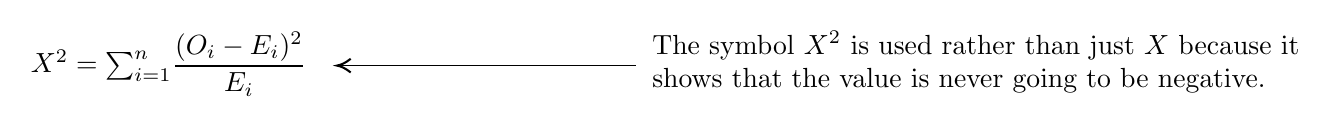
\begin{tikzpicture}[x=0.75pt,y=0.75pt,yscale=-1,xscale=0.6]
        % Shape: Boxed Line [id:dp5924871900366302] 
        \draw (490,21) -- (250,21) ;
        \draw [shift={(250,21)}, rotate = 360.07] [color=black][line width=0.75]    (10.93,-3.29) .. controls (6.95,-1.4) and (3.31,-0.3) .. (0,0) .. controls (3.31,0.3) and (6.95,1.4) .. (10.93,3.29)   ;
        
        % Text Node
        \draw (2,3.4) node [anchor=north west][inner sep=0.75pt]{%
            $X^{2} ={\mathlarger\sum _{i=1}^{n}}\dfrac{( O_{i} -E_{i})^{2}}{E_{i}}$
        };
        
        % Text Node
        \draw (501,3) node [anchor=north west][inner sep=0.75pt][align=left]{%
            The symbol $\displaystyle X^{2}$ is used rather than just $\displaystyle X$ because it\\
            shows that the value is never going to be negative.};
    \end{tikzpicture}
    
    You can see that the less good the fit, the larger the difference between each observed and expected value, and the greater the value of $X^2$.
    
    
    \textbf{Here is another way of calculating $X^2$:}
    
    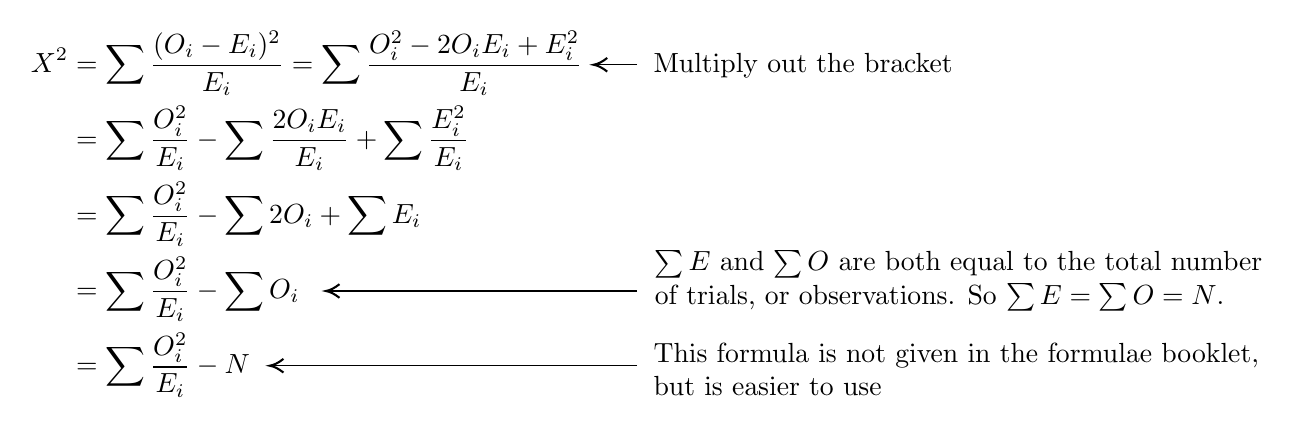
\begin{tikzpicture}[x=0.75pt,y=0.75pt,yscale=-1,xscale=0.6]
        % Uncomment if require:
        % \path (0,354);  % Set diagram left start at 0, and has height of 354
        
        % Straight Lines [id:da18451996657129888] 
        \draw (490,102) -- (455,102) ;
        \draw [shift={(455,102)}, rotate = 360] [color=black][line width=0.75]    (10.93,-3.29) .. controls (6.95,-1.4) and (3.31,-0.3) .. (0,0) .. controls (3.31,0.3) and (6.95,1.4) .. (10.93,3.29)   ;
        % Straight Lines [id:da645763229182968] 
        \draw (490,211) -- (240,211) ;
        \draw [shift={(240,211)}, rotate = 360] [color=black][line width=0.75]    (10.93,-3.29) .. controls (6.95,-1.4) and (3.31,-0.3) .. (0,0) .. controls (3.31,0.3) and (6.95,1.4) .. (10.93,3.29)   ;
        % Straight Lines [id:da09218839837294457] 
        \draw (490,247) -- (195,247) ;
        \draw [shift={(195,247)}, rotate = 360] [color=black][line width=0.75]    (10.93,-3.29) .. controls (6.95,-1.4) and (3.31,-0.3) .. (0,0) .. controls (3.31,0.3) and (6.95,1.4) .. (10.93,3.29)   ;
        
        
        % Text Node
        \draw (1,84.4) node [anchor=north west][inner sep=0.75pt]{
            $\begin{aligned}
                X^{2} & =\sum \dfrac{( O_{i} -E_{i})^{2}}{E_{i}} =\sum \dfrac{O_{i}^{2} -2O_{i} E_{i} +E_{i}^{2}}{E_{i}}\\
                      & =\sum \dfrac{O_{i}^{2}}{E_{i}} -\sum \dfrac{2O_{i} E_{i}}{E_{i}} +\sum \dfrac{E_{i}^{2}}{E_{i}}\\
                      & =\sum \dfrac{O_{i}^{2}}{E_{i}} -\sum 2O_{i} +\sum E_{i}\\
                      & =\sum \dfrac{O_{i}^{2}}{E_{i}} -\sum O_{i}\\
                      & =\sum \dfrac{O_{i}^{2}}{E_{i}} -N
            \end{aligned}$
        };
        
        % Text Node
        \draw (501,95) node [anchor=north west][inner sep=0.75pt][align=left]{%
            Multiply out the bracket
        };
        % Text Node
        \draw (502,190) node [anchor=north west][inner sep=0.75pt][align=left]{%
            $\sum E$ and $\sum O$ are both equal to the total number \\
            of trials, or observations. So $\sum E=\sum O=N$.
        };
        % Text Node
        \draw (501,235) node [anchor=north west][inner sep=0.75pt][align=left]{%
            This formula is not given in the formulae booklet,\\but is easier to use
        };
    \end{tikzpicture}
\end{mybox2}
\newpage













\begin{examplebox}{}{}
    \\ % TODO Example 1
    Billy and Mel each have two 4-sided spinners numbered 1-4. They each carry out experiments where they spin their spinners at the same time and add the scores together. After each student has carried out 160 experiments, the frequency distributions are as follows:

    \begin{center}
    \begin{minipage}[t]{0.9\linewidth}
        \begin{tabularx}{\textwidth}{|X|*7{P{11mm}|}}
            \hline
            \textbf{Number, n} & 2 & 3 & 4 & 5 & 6 & 7 & 8                          \\\hline
            \textbf{Observed by Billy ($O_i$)} & 12 & 15 & 22 & 41 & 33 & 21 & 16   \\\hline
            \textbf{Observed by Mel ($O_i$)} & 6 & 12 & 21 & 37 & 35 & 29 & 20      \\\hline
        \end{tabularx}
        \vspace{4mm}
    \end{minipage}
    \end{center}
    
    \begin{enumerate}[label*=\bfseries (\alph*), leftmargin=*]
        \item[] Both Billy and Mel believe that their spinners are fair.
        \item State the null and alternative hypothesis for this experiment \vspace{3mm}
        \item[] One of the students has a biased spinner. 
        \item Calculate the goodness-of-fit test statistic for both students and determine which of them is most likely to have a biased spinner.
    \end{enumerate}
\end{examplebox}
\vfill

\begin{practice*}{Exercise 6A}{}
\end{practice*}

\newpage

\subsection{Testing a Hypothesis}

\begin{examplebox}{}{}
    \\ % TODO Example 2
    In an experiment a die is rolled 120 times.
    
    \begin{center}
    \begin{minipage}[t]{0.8\linewidth}
        \begin{tabularx}{\textwidth}{|X|*6{P{11mm}|}}
            \hline
            \textbf{Number on dice, n} & 1 & 2 & 3 & 4 & 5 & 6                      \\\hline
            \textbf{Observed frequency ($O_i$)} & 23 & 15 & 25 & 18 & 21 & 18       \\\hline
        \end{tabularx}
        \vspace{4mm}
    \end{minipage}
    \end{center}
    
    Test, at the 5\% significance level, whether or not the number showing on the die when it is rolled could be modelled by a discrete uniform distribution.

\end{examplebox}
\newpage



\begin{examplebox}{}{}
    \\ % TODO Example 3
    A school conducted a survey into the impact that a new exercise club was having on students. Prior to the new club starting, 60\% of students said they had no regular exercise, 30\% reported exercising once a week and 10\% reported exercising more than once a week. After the new club started, they surveyed the 150 students to find out how often they exercised.    
    
    \begin{center}
    \begin{minipage}[t]{\linewidth}
        \begin{tabularx}{\textwidth}{|X|P{38mm}|P{27mm}|P{44mm}|P{20mm}|}
            \cline{2-5}
            \multicolumn{1}{c|}{} & \textbf{No regular exercise} & \textbf{Once a week} & \textbf{More than once a week} & \textbf{Total}  \\\hline
            \textbf{Frequency}    & 73                           & 57                   & 20                             & 150             \\\hline
        \end{tabularx}
        \vspace{4mm}
    \end{minipage}
    \end{center}
    
    Based on these data, is there evidence of a change in attitude to exercise following the introduction of the new club? Test the data at a 5\% significance level.

\end{examplebox}
\newpage



\begin{examplebox}{}{}
    \\ % TODO Example 4
    It is suggested that 40\% of households have 0 children, 20\% have 1 child, 25\% have 2 children, 10\% have 3 children and 5\% have 4 or more children. \vspace{2mm}\\
    The table below shows the observed frequencies for a sample of 80 households.
    
    \begin{center}
        \begin{minipage}[t]{0.9\linewidth}
            \begin{tabularx}{\textwidth}{|X|*5{P{16mm}|}}
                \hline
                \textbf{Number of children, n}      & 0  & 1  & 2  & 3 & $\geq$ 4 \\\hline
                \textbf{Observed frequency ($O_i$)} & 27 & 19 & 27 & 4 & 3        \\\hline
                \textbf{Expected frequency ($E_i$)} &    &    &    &   &          \\\hline
            \end{tabularx}
            \vspace{4mm}
        \end{minipage}
    \end{center}
    
    Test at the 5\% significance level whether or not the suggested distribution is a suitable model.
\end{examplebox}
\vfill
\begin{practice*}{Exercise 6B}{}
\end{practice*}
\newpage



\lesson{Testing with Discrete Distributions (Parameter Known)}

\begin{mybox2}[colbacktitle=WildStrawberry]{Summary}
    \begin{enumerate}[leftmargin=5.5mm, rightmargin=4mm]
        \item Determine which distribution is likely to be a good model by examining the conditions applying to the observed data.
        \item Set the significance level, for example 5\%.
        \item Estimate parameters (if necessary) from your observed data.
        \item Form your hypotheses.
        \item Calculate expected frequencies.
        \item Combine any expected frequencies so that none are less than 5.
        \item Find $v$ using $v$ = number of cells after combining -- number constraints or restrictions.
        \item Find the critical value $\chi^2$ from the table.
        \item Calculate ${\mathlarger\sum}\dfrac{(O_i-E_i)^2}{E_i}$ or ${\mathlarger\sum}\dfrac{O_i^2}{E_i}-N$.
        \item See if your value is significant.
        \item Draw the appropriate conclusion and interpret in the context of the original problem.
    \end{enumerate}    
\end{mybox2}
\begin{examplebox}{}{}
    \\ % TODO Example 5
    The data in the table are thought to be modelled by a binomial distribution $B(10,0.2)$.
    
    \begin{center}
        \begin{minipage}[t]{0.75\linewidth}
            \begin{tabularx}{\textwidth}{|X|*9{P{8mm}|}}
                \hline
                $x$                & 0  & 1  & 2  & 3  & 4 & 5 & 6 & 7 & 8    \\\hline
                \textbf{Frequency} & 12 & 28 & 28 & 17 & 7 & 4 & 2 & 2 & 0    \\\hline
            \end{tabularx}
            \vspace{4mm}
        \end{minipage}
    \end{center}
    
    Test, at the 5\% significance level, whether this is a good model.
\end{examplebox}
\newpage

\begin{examplebox}{}{}
    \\ % TODO Example 6
    The number of telephone calls arriving at an exchange in six-minute periods were recorded over a period of 8 hours, with the following results.
    
    \begin{center}
    \begin{minipage}[t]{0.8\linewidth}
        \begin{tabularx}{\textwidth}{|X|*9{P{8mm}|}}
            \hline
            \textbf{Number of calls, $r$} & 0 & 1  & 2  & 3  & 4 & 5 & 6 & 7 & 8    \\\hline
            \textbf{Frequency, $f_r$}     & 8 & 19 & 26 & 13 & 7 & 5 & 1 & 1 & 0    \\\hline
        \end{tabularx}
        \vspace{4mm}
    \end{minipage}
    \end{center}
    
    Can these results be modelled using the Poisson distribution with mean 2.2. \\Show how you decide using a 5\% level of significance.
\end{examplebox}\vspace{1mm}
\begin{minipage}[t]{\linewidth}
    \renewcommand{\arraystretch}{1.5}%
    \begin{tabularx}{\textwidth}{|X|*9{P{12mm}|}}
        \hline
        \cellcolor[HTML]{E0E0E0}\textbf{Number of calls}    & 0     & 1      & 2      & 3      & 4     & 5 & 6 & 7 & \\\hline
        \cellcolor[HTML]{E0E0E0}\textbf{Probability}        &       &        &        &        &       &   &   &   & \\\hline
        \cellcolor[HTML]{E0E0E0}\textbf{Expected frequency} & 8.864 & 19.501 & 21.451 & 15.731 & 8.652 &   &   &   & \\\hline
    \end{tabularx}
    \vspace{4mm}
\end{minipage}

\newpage

\begin{examplebox}{}{}
    \\
    Sarah has a large DVD collection. Every week she picks DVDs off the shelf at random until she finds one she would like to watch. Sarah thinks that there is about a 50\% chance she will be in the mood to watch any particular DVD. Over the course of a year she records the number of DVDs she picks off the shelf before finding one she would like to watch. The results are recorded in the frequency table below.
    
    \begin{center}
    \begin{minipage}[t]{0.7\linewidth}
        \begin{tabularx}{\textwidth}{|X|*6{>{\centering\arraybackslash}p{10mm}|}}
            \hline
            \textbf{Number of DVDs}             & 1  & 2  & 3 & 4 & \textbf{Total} \\\hline
            \textbf{Observed frequency ($O_i$)} & 33 & 12 & 5 & 2 & 52             \\\hline
        \end{tabularx}
        \vspace{4mm}
    \end{minipage}
    \end{center}
    
    \begin{enumerate}[label*=\bfseries (\alph*), leftmargin=*]
        \item Calculate the expected frequencies if the number of DVDs considered is modelled as Geo(0.5) random variable. \vspace{2mm}
        \item[] Sarah wants to check if her guess that there is a 50\% chance she'll watch any particular DVD is supported by the data. 
        \item Formulate the null and alternative hypotheses.
        \item Is Sarah right in her assumption? Test at the 5\% significance level.
    \end{enumerate}

\end{examplebox}
\vfill
\begin{practice*}{Exercise 6C}{}
\end{practice*}
\newpage

\lesson{Testing with Discrete Distributions (Parameter Not Known)}
\begin{mybox2}[colbacktitle=WildStrawberry]{Summary}
    \begin{itemize}[leftmargin=5.5mm]
        \item For any sample of a random variable $X$, $E(\overline{X}) = E(X)$.
        \item This means that for a sample, as the sample size increases, $\overline{X} \rightarrow E(X)$.
        \item This means that we can approximate $\overline{X} \approx E(X)$.
        \item We can use this fact to estimate unknown parameters of a distribution.
    \end{itemize}
    
    \textbf{Poisson} \\
    If $ X\sim \text{\rmfamily Po}(\lambda)$, the sample mean $X \approx \lambda$. \\
    
    \textbf{Binomial} \\
    If $X \sim \text{\rmfamily B}(n, p)$, the sample mean $\overline{X} \approx np$, \hspace{5mm}$p\approx \dfrac{\overline{X}}{n}$ \\
    
    \textbf{Geometric} \\
    If $X \sim \text{\rmfamily B}(p)$, the sample mean $\overline{X} \approx \dfrac{1}{p}$, \hspace{10mm}$p\approx \dfrac{1}{\overline{X}}$
\end{mybox2}

\begin{examplebox}{}{}
    \\
    A study of the number of girls in families with five children was done on 100 such families.\\
    The results are summarised in the following table.
    
    \begin{center}
    \begin{minipage}[t]{0.7\linewidth}
        \begin{tabularx}{\textwidth}{|X|*7{>{\centering\arraybackslash}p{10mm}|}}
            \hline
            \textbf{Number of girls (r)} & 0 & 1 & 2 & 3 & 4 & 5                          \\\hline
            \textbf{Frequency} & 13 & 18 & 38 & 20 & 10 & 1       \\\hline
        \end{tabularx}
        \vspace{4mm}
    \end{minipage}
    \end{center}
    
    Test at the 5\% significance level, whether or not the binomial distribution is a suitable model for the data.
\end{examplebox}
\newpage



\begin{examplebox}{}{}
    \\ % TODO Example 9
    Breakdowns on a certain stretch of motorway were recorded each day for 80 consecutive days. The results are summarised in the table below.
    
    \begin{center}
    \begin{minipage}[t]{0.6\linewidth}
        \begin{tabularx}{\textwidth}{|X|*4{>{\centering\arraybackslash}p{10mm}|}}
            \hline
            \textbf{Number of breakdowns} & 0 & 1 & 2 & >2                          \\\hline
            \textbf{Frequency} & 38 & 32 & 10 & 0       \\\hline
        \end{tabularx}
        \vspace{4mm}
    \end{minipage}
    \end{center}
    
    It is suggested that the number of breakdowns per day can be modelled by a Poisson distribution. \vspace{2mm}\\
    Using 5\% significance level, test whether or not the Poisson distribution is a suitable model for these data. State your hypotheses clearly.\hfill\textbf{(9 marks)}
\end{examplebox}
\newpage



\begin{examplebox}{}{}
    \\ % TODO Example 10
    David doesn't have a car. If it's raining in the morning when he has to go to work, he calls his friends one by one to see if anyone can give him a lift. Since starting his job it has rained on 255 mornings. \\David has recorded the number of calls he had to make on each of these morning before finding a willing driver.
    
    \begin{center}
    \begin{minipage}[t]{0.8\linewidth}
        \begin{tabularx}{\textwidth}{|X|*9{>{\centering\arraybackslash}p{10mm}|}}
            \hline
            \textbf{Number of calls} & 1   & 2  & 3  & 4  & 5  & 6 & 7 & \textbf{Total}  \\\hline
            \textbf{Frequency}       & 130 & 54 & 24 & 28 & 13 & 5 & 1 & 255             \\\hline
        \end{tabularx}
        \vspace{4mm}
    \end{minipage}
    \end{center}
    
    Assume that each of David's friends is equally likely to offer him a lift, and that David will \\never run out of friends to call. (David is extremely popular.)
    \begin{enumerate}[label*=\bfseries (\alph*), leftmargin=*]
        \item Suggest a suitable distribution to model the number of calls made by David on\\ a rainy morning.  \hfill\textbf{(1 mark)}
        \item Use the observed data to estimate any parameters necessary for your \\chosen distribution.        \hfill\textbf{(2 marks)}
        \item Carry out a goodness-of-fit test at the 5\% significance level for your chosen \\distribution.    \hfill\textbf{(6 marks)}
    \end{enumerate}
\end{examplebox}

\textbf{Use this table in part (c):}\vspace{2mm}

\begin{minipage}[t]{0.9\linewidth}
    %\setstretch{1.5}
    \renewcommand{\arraystretch}{1.5}%
    \begin{tabularx}{\textwidth}{|X|*9{>{\centering\arraybackslash}p{12mm}|}}
        \hline
        \cellcolor[HTML]{E0E0E0}\textbf{Number of calls}  & 1      & 2     & 3     & 4     & 5    & 6 & 7 & \textbf{Total} \\\hline
        \cellcolor[HTML]{E0E0E0}\textbf{Observed ($O_i$)} & 130    & 54    & 24    & 28    & 13   &   &   & 60             \\\hline
        \cellcolor[HTML]{E0E0E0}\textbf{Expected ($E_i$)} & 124.09 & 63.70 & 32.70 & 16.79 & 8.62 &   &   & 60             \\\hline
    \end{tabularx}
    \vspace{4mm}
\end{minipage}
\newpage

\begin{note*}{\hspace{-3.5mm}}
    If the distribution you are testing is the discrete uniform distribution, then you have not estimated any \\parameters.    
\end{note*}
\begin{examplebox}{}{}
    \\ % TODO Example 11
    Successful contestants in a TV game show were allowed to select from one of five boxes, four of which contained prizes, and one of which contained nothing. The boxes were numbers 1 to 5, and, when the show had run for 100 weeks, the choices made by the contestants were analysed with the following results:
    \begin{center}
    \begin{minipage}[t]{0.55\linewidth}
        \begin{tabularx}{\textwidth}{|X|*5{>{\centering\arraybackslash}p{10mm}|}}
            \hline
            \textbf{Box number} & 1  & 2  & 3  & 4  & 5        \\\hline
            \textbf{Frequency}  & 20 & 16 & 25 & 18 & 21       \\\hline
        \end{tabularx}
        \vspace{4mm}
    \end{minipage}
    \end{center}
    
    \begin{enumerate}[label*=\bfseries (\alph*), leftmargin=*]
        \item Explain why these data could possibly be modelled by a discrete uniform distribution.
        \item Using a significance level 5\%, test to see if the discrete uniform distribution is a good model \\in this particular case.    
    \end{enumerate}

\end{examplebox}
\vfill
\begin{practice*}{Exercise 6D}{}
\end{practice*}
\newpage

\lesson{Using Contingency Tables}
\begin{mybox2}[colbacktitle=WildStrawberry]{Summary}
    \bfseries
    \begin{itemize}[leftmargin=5.5mm]
        \setlength\itemsep{1em}
        \item Expected frequency = $\dfrac{\text{row total}\times\text{column total}}{\text{grand total}}$
        \item The number of degrees of freedom\\
            $v=(h-1)(k-1)$ \mdseries\hspace{3cm}where $h$ = number of rows and $k$ = number of columns.
    \end{itemize}
\end{mybox2}
\begin{examplebox}{}{}
    \\ % TODO Example 12
    Test, at the 5\% significance level, whether or not the school that a pupil attends and their grade are independent.
    
    \begin{center}
    \begin{minipage}[t]{0.7\linewidth}
        \renewcommand{\arraystretch}{1.2}
        \begin{tabularx}{\textwidth}{|X|P{10mm}|*3{P{15mm}|}P{20mm}|}
            \hhline{~~|---|-|}
            \multicolumn{2}{c|}{} & \multicolumn{3}{c|}{\cellcolor[HTML]{E0E0E0}Pass (criterion 1)}                            & \cellcolor[HTML]{E0E0E0}   \\\hhline{~~|---|>{\arrayrulecolor[HTML]{E0E0E0}}->{\arrayrulecolor{black}}|}
            \multicolumn{2}{c|}{} & \cellcolor[HTML]{E0E0E0}$A$  & \cellcolor[HTML]{E0E0E0}$B$  & \cellcolor[HTML]{E0E0E0}$C$  & \cellcolor[HTML]{E0E0E0}\multirow{-2}{*}{Totals}  \\\hline
            \cellcolor[HTML]{E0E0E0} & \cellcolor[HTML]{E0E0E0}$X$ & 18 & 12 & 20 & 50                                                                      \\\hhline{|>{\arrayrulecolor[HTML]{E0E0E0}}->{\arrayrulecolor{black}}|*5{-}|}
            \multirow{-2}{=}{\cellcolor[HTML]{E0E0E0}\shortstack[l]{School\\(criterion 2)}} & \cellcolor[HTML]{E0E0E0}$Y$ & 26 & 12 & 32 & 70               \\\thickhline
            \cellcolor[HTML]{E0E0E0} Totals & \cellcolor[HTML]{E0E0E0} & 44 & 24 & 52 & 120                                                                 \\\hline          
        \end{tabularx}
        \vspace{4mm}
    \end{minipage}
    \end{center}
\end{examplebox}
\newpage

\begin{examplebox}{}{}
    \\ % TODO Example 13
    During the trial of a new drug, 60 volunteers out of 200 were treated with the drug. Those who experienced relief of their symptoms and those who did not were recorded a in the table.
    
    \begin{center}
    \begin{minipage}[t]{0.6\linewidth}
        \begin{tabularx}{\textwidth}{|X|*3{P{20mm}|}}
            \cline{2-4}
            \multicolumn{1}{c|}{} & \textbf{Relief} & \textbf{No relief} & \textbf{Totals}   \\\hline
            \textbf{Treated}      & 10              & 50                 & 60                \\\hline
            \textbf{Not Treated}  & 40              & 100                & 140               \\\hline
            \textbf{Totals}       & 50              & 150                & 200               \\\hline
        \end{tabularx}
        \vspace{4mm}
    \end{minipage}
    \end{center}
    
    Use a suitable test to see if there is any association between treatment with the drug and relief of symptoms. Use a 5\% significance level.
\end{examplebox}
\vfill
\begin{practice*}{Exercise 6E}{}
\end{practice*}
\newpage


\fakesubsection{Exercises}
\exercise{}
\begin{enumerate}
    \setlength\itemsep{0.5em}
    \item An octagonal dice is thrown 500 times and the results are noted. It is assumed that the dice is unbiased. A test is to be done to see whether the observed results differ from the expect ones. \\Write down a null hypothesis and an alternative hypothesis that can be used.
    
    \item A six-sided dice is rolled 180 times to try to establish whether or not it is fair. The results of the rolls are as follows:\vspace{3mm}\\
        \begin{tabularx}{0.65\textwidth}{|X|*6{>{\centering\arraybackslash}p{10mm}|}}
            \hline
            \textbf{Number, $n$}            & 1  & 2  & 3  & 4  & 5  & 6        \\\hline
            \textbf{Observed rolls ($O_i$)} & 27 & 33 & 31 & 28 & 34 & 27       \\\hline
        \end{tabularx}\vspace{6mm}
        \begin{enumerate}[label=\bfseries \alph*\space ]
            \item State suitable null and alternative hypotheses for the experiment
            \item Calculate $X^2$ for the observed data.
        \end{enumerate}
        
    \item A random sample of 750 UK secondary school students is taken, and the year group they are each in is recorded:\vspace{3mm}\\
        \begin{tabularx}{0.58\textwidth}{|X|*5{>{\centering\arraybackslash}p{10mm}|}}
            \hline
            \textbf{Year}                   & 7 & 8 & 9 & 10 & 11               \\\hline
            \textbf{Observed rolls ($O_i$)} & 190 & 145 & 145 & 140 & 130       \\\hline
        \end{tabularx}\vspace{6mm}
        \begin{enumerate}[label=\bfseries \alph*\space ]
            \item State suitable null and alternative hypotheses
            \item Calculate the expected number of students in each year group assuming your null hypothesis is true.
            \item Calculate $X^2$ for the observed data.
        \end{enumerate}
        
    \item A particular genetic mutation is believed to have a 75\% chance of being passed from parent to child. In an experiment, 160 adults with the mutation each had one of their children tested to see if the child had inherited the mutation. The results are as follows:\vspace{3mm}\\
        \begin{tabularx}{0.37\textwidth}{|X|*2{>{\centering\arraybackslash}p{10mm}|}}
            \hline
            \textbf{Mutation present} & Yes & No  \\\hline
            \textbf{Observed ($O_i$)} & 117 & 43  \\\hline
        \end{tabularx}\vspace{6mm}
        \begin{enumerate}[label=\bfseries \alph*\space ]
            \item Calculate the expected frequencies
            \item State the null and alternative hypotheses.
            \item Calculate the goodness of fit of the data to the expected result.
        \end{enumerate}
        
    \item John has two coins that he can't tell apart. One is fair. The other is biased and will land on heads with probability 0.6. He flips one of the coins 50 times and records the results in the frequency table given below.\vspace{3mm}\\
        \begin{tabularx}{0.37\textwidth}{|X|*2{>{\centering\arraybackslash}p{10mm}|}}
            \hline
            \textbf{Result}           & H  & T   \\\hline
            \textbf{Observed ($O_i$)} & 28 & 22  \\\hline
        \end{tabularx}\vspace{6mm}
        \begin{enumerate}[label=\bfseries \alph*\space ]
            \item Calculate the expected frequencies for each coin
            \item Calculate the goodness of fit between the observed results and the expected results for each coin.
            \item Which coin is John more likely to have been using? Give a reason for your answer.
        \end{enumerate}
        
    \item The BMI profile of English adults is given below. \vspace{2mm}\\
        \begin{tabularx}{0.89\textwidth}{|X|*5{>{\centering\arraybackslash}p{22mm}|}}
            \hline
            \textbf{Country} & Underweight  & Normal & Overweight & Obese & Total   \\\hline
            England          & 2\%          & 35\%   & 36\%       & 27\%  & 100\%   \\\hline
        \end{tabularx}\vspace{4mm}
        
        {\footnotesize\hfill Obesity Statistics, House of Commons Briefing Paper, Number 336, 2017\hspace{0.06\textwidth}}\vspace{2mm}
        
        You may assume that these percentages reflect the true distribution. A sample is taken of adults in Wales, and the results are recorded in the table below.\vspace{2mm}\\
        \begin{tabularx}{0.89\textwidth}{|X|*5{>{\centering\arraybackslash}p{22mm}|}}
            \hline
            \textbf{Country} & Underweight  & Normal & Overweight & Obese & Total   \\\hline
            Wales (Men)      & 4            & 70     & 80         & 46    & 200     \\\hline
            Wales (Women)    & 6            & 81     & 65         & 48    & 200     \\\hline
        \end{tabularx}\vspace{6mm}
        
        By calculating the goodness-of-fit statistic for both Welsh men and women, determine which group more closely matches the English distribution.
\end{enumerate}
\newpage

\exercise{}
\begin{enumerate}
    \setlength\itemsep{0.5em}
    \item In an experiment where a dice is rolled 72 times, the frequency distribution is to be compared to a discrete uniform distribution as shown:\vspace{3mm}\\
        \begin{tabularx}{0.7\textwidth}{|X|*6{>{\centering\arraybackslash}p{10mm}|}}
            \hline
            \textbf{Number on dice, $n$}       & 1  & 2  & 3  & 4  & 5  & 6       \\\hline
            \textbf{Observed frequency, $O_i$} & 16 & 11 & 13 & 15 & 8  & 9       \\\hline
            \textbf{Expected frequency, $E_i$} & 12 & 12 & 12 & 12 & 12 & 12      \\\hline
        \end{tabularx}\vspace{5mm}
        
        Test, at the 5\% significance level, whether or not the observed frequencies could be modelled by a discrete uniform distribution. \hfill\textbf{(6 marks)}
    \item In a tombola, tickets ending in 0 or a 5 are guaranteed a prize.  \\
        All other tickets will lose. At a fair, 120 tickets were drawn, and \\ 
        the numbers of winning tickets were as follows.                     \vspace{4mm}\\
        \begin{tabularx}{0.55\textwidth}{|X|*3{>{\centering\arraybackslash}p{15mm}|}}
            \cline{2-4}
            \multicolumn{1}{c|}{}          & Winning & Losing & Total \\\hline
            \textbf{Observed ticket draws} & 15      & 105    & 120   \\\hline
        \end{tabularx}
        \begin{table}[!ht]
            \begin{tabularx}{\dimexpr\textwidth}{Xp{2.0in}}
                {} & \vspace{-3.5cm}\begin{mybox2}[colbacktitle=green]{Hint}
                    If the tickets were fairly\\ distributed, it would be \\expected that 2 in every 10 would be winning tickets.
                \end{mybox2}
            \end{tabularx}
        \end{table}\vspace{-2mm}
        
        Test, at the 5\% significance level, whether or not the tombola was fair \hfill\textbf{(6 marks)}
    \item A local travel agent has made a prediction as to how many trips abroad his customers make. He surveys a sample of 100 customers and compares the results to his expectations.\vspace{2mm}\\
        \begin{tabularx}{0.6\textwidth}{|X|*3{>{\centering\arraybackslash}p{22mm}|}}
            \hline
            \textbf{Trips abroard} & None & One  & Two or more   \\\hline
            \textbf{Expected}      & 10\% & 60\% & 30\%          \\\hline
            \textbf{Sample}        & 4    & 73   & 23            \\\hline
        \end{tabularx}\vspace{5mm}
        
        Test, at the 2.5\% significance level, whether the travel agent's prediction firs the observed data.
        
        \vspace{-1.2mm}\hfill\textbf{(6 marks)}
    \item In a sample of 100 households, the actual and expected numbers    \\
        of dogs is a follows:                                               \vspace{3mm}\\
        \begin{tabularx}{0.61\textwidth}{|X|*7{>{\centering\arraybackslash}p{8mm}|}>{\centering\arraybackslash}p{11mm}|}
            \hline
            \textbf{Dogs}     & 0  & 1  & 2  & 3 & 4 & 5 & >5 & \textbf{Total} \\\hline
            \textbf{Observed} & 45 & 19 & 11 & 8 & 7 & 6 & 4  & 100            \\\hline
            \textbf{Expected} & 55 & 20 & 10 & 7 & 4 & 3 & 1  & 100            \\\hline
        \end{tabularx}\vspace{6mm}\\
        \begin{minipage}{0.59\textwidth}
        \begin{enumerate}[label=\bfseries \alph*\space ]
            \item Explain why there are 4 degrees of freedom in \\this case.\hfill\textbf{(2 marks)}
            \item Test, at the 5\% significance level, whether the observed data fits the expected distribution given.\hfill\textbf{(5 marks)}
        \end{enumerate}
        \end{minipage}
        \begin{table}[!ht]
            \begin{tabularx}{\dimexpr\textwidth}{Xp{2.17in}}
                {} & \vspace{-6.1cm}\begin{mybox2}[colbacktitle=green]{Problem-solving}
                    When using a $\chi^2$ distribution to approximate the \\distribution of $X^2$, if any of the expected frequencies is less than 5 you need to combine cells.
                \end{mybox2}
            \end{tabularx}
        \end{table}\vspace{-6mm}
    \item In the year 2000, the birth weights of babies were distributed as follows:\vspace{2mm}\\
        \begin{tabularx}{0.945\textwidth}{|X|*9{>{\centering\arraybackslash}p{17mm}|}}
            \hline
            \textbf{Weight (g)} & \textbf{Under 1500}  & \textbf{1500-1999} & \textbf{2000-2499} & \textbf{2500-2999} & \textbf{3000-3499} & \textbf{3500 and over} & \textbf{Total} \\\hline
            \textbf{Percentage} & 1.3\%          & 1.5\%        & 5\%        & 16.5\%         & 35.7\%         & 40\%             & 100\%            \\\hline
        \end{tabularx}\vspace{6mm}\\
        In the year 2015, the birth weights of babies were as follows:\vspace{2mm}\\
        \begin{tabularx}{0.945\textwidth}{|X|*9{>{\centering\arraybackslash}p{17mm}|}}
            \hline
            \textbf{Weight (g)} & \textbf{Under 1500}  & \textbf{1500-1999} & \textbf{2000-2499} & \textbf{2500-2999} & \textbf{3000-3499} & \textbf{3500 and over} & \textbf{Total} \\\hline
            \textbf{Frequency}  & 7286          & 9304        & 32 121        & 112 535         & 244 472         & 281 942             & 687 600            \\\hline
        \end{tabularx}\vspace{6mm}\\
        Using a 5\% significance level, decide whether the distribution of birth weights from 2000 can be used as a model for the weights in 2015. \hfill\textbf{(8 marks)}
\end{enumerate}
\newpage
\exercise{}

\begin{enumerate}
    \setlength\itemsep{0.5em}
    \item The following table shows observed values for a distribution which it is though may be modelled by a Poisson distribution.\vspace{3mm}\\
        \begin{tabularx}{0.7\textwidth}{|X|*7{>{\centering\arraybackslash}p{11mm}|}}
            \hline
            \textbf{$x$}       & 0  & 1  & 2  & 3  & 4  & 5 & >5       \\\hline
            \textbf{Frequency} & 12 & 23 & 24 & 24 & 12 & 5 & 0       \\\hline
        \end{tabularx}\vspace{6mm}\\
        A possible model is thought to be Po(2). From tables, the expected values are found to be as shown in the following table.\vspace{2mm}\\
        \begin{tabularx}{0.85\textwidth}{|X|*7{>{\centering\arraybackslash}p{11.5mm}|}}
            \hline
            \textbf{$x$}                       & 0     & 1     & 2     & 3     & 4     & 5    & >5         \\\hline
            \textbf{Expected frequency of $x$} & 13.53 & 27.07 & 27.07 & 18.04 & 9.02  & 3.61 & 1.66       \\\hline
        \end{tabularx}\vspace{4mm}\\
        \begin{enumerate}[label=\bfseries \alph*\space ]
            \item Conduct a goodness-of-fit test at the 5\% significance level.
        \end{enumerate}
    \item A mail-order firm receives packets every through the mail.
    
        They think that their deliveries are uniformly distributed throughout the week. Test this assertion given that their deliveries over a four-week period were as follows. Use a 0.05 significance level.\vspace{2mm}\\
        \begin{tabularx}{0.6\textwidth}{|X|*6{>{\centering\arraybackslash}p{11mm}|}}
            \hline
            \textbf{Day}       & Mon & Tue & Wed & Thu & Fri  & Sat   \\\hline
            \textbf{Frequency} & 15  & 23  & 19  & 20  & 14   & 11    \\\hline
        \end{tabularx}\vspace{3mm}\\
    \item Data were collected on the number of female puppies born in 200 litters of 8 puppies. It was decided to test whether or not a binomial model with parameters $n$ = 8 and $p$ = 0.5 is a suitable model for the data. The following table shows the observed frequencies and the expected frequencies, to 2 decimal places, obtained in order to carry out this test.\vspace{2mm}\\
        \begin{tabular}{|P{43mm}|*2{P{52mm}|}}
            \hline
            \textbf{Number of females} & \textbf{Observed number of litters} & \textbf{Expected number of litters} \\\hline
            0                          & 1                                   & 0.78                                \\\hline
            1                          & 9                                   & 6.25                                \\\hline
            2                          & 27                                  & 21.88                               \\\hline
            3                          & 46                                  & $R$                                 \\\hline
            4                          & 49                                  & $S$                                 \\\hline
            5                          & 35                                  & $T$                                 \\\hline
            6                          & 26                                  & 21.88                               \\\hline
            7                          & 5                                   & 6.25                                \\\hline
            8                          & 2                                   & 0.78                                \\\hline
        \end{tabular}\vspace{2mm}
        \begin{enumerate}[label=\bfseries \alph*\space ]
            \item Find the values of $R$, $S$ and $T$. \hfill\textbf{(3 marks)}
            \item Carry out the test to determine whether or not this binomial model is a suitable one. \\
                State your hypotheses clearly and use a 5\% level of significance. \hfill\textbf{(5 marks)}
        \end{enumerate}
    \item The following table shows observed values for what is though to be a geometric distribution with $p$ = 0.6.\vspace{2mm}\\
        \begin{tabularx}{0.8\textwidth}{|X|*7{>{\centering\arraybackslash}p{10.5mm}|}}
            \hline
            \textbf{$k$}                        & 1   & 2  & 3  & 4 & 5 & 6 & \textbf{Total} \\\hline
            \textbf{Observed frequency ($O_k$)} & 207 & 66 & 13 & 9 & 3 & 2 & 300            \\\hline
        \end{tabularx}\vspace{5mm}
        
        Calculate the expected frequencies and, using a 1\% significance level, conduct a \\goodness-of-fit test. \hfill\textbf{(6 marks)}
    \item The following table shows observed values for what is though to be a geometric distribution with $p$ = 0.4.\vspace{2mm}\\
        \begin{tabularx}{0.8\textwidth}{|X|*7{>{\centering\arraybackslash}p{10.5mm}|}}
            \hline
            \textbf{$k$}                        & 1   & 2  & 3  & 4 & 5 & 6 & \textbf{Total} \\\hline
            \textbf{Observed frequency ($O_k$)} & 207 & 66 & 13 & 9 & 3 & 2 & 300            \\\hline
        \end{tabularx}\vspace{5mm}
        
        Calculate the expected frequencies and, using a 5\% significance level, conduct a \\goodness-of-fit test. \hfill\textbf{(6 marks)}
    \newpage
    \item Michael has a pet monkey and wants to test the theory that, given a typewriter in enough time, the monkey will eventually type out the complete works of Shakespeare. Unfortunately, the experiment is a total disaster, and the monkey has succeeded only in producing a seemingly random string of alphabetic characters!
        
        Michael decides instead he will see how random the string of characters is. He reads the string looking for vowels. Each time he finds a vowel, he counts the number of letters until the next vowel. The results are recorded in the table below.\vspace{3mm}\\
        \begin{tabularx}{0.9\textwidth}{|X|*7{P{7mm}|}P{16mm}|P{12mm}|}
            \hline
            \textbf{Characters to the next vowel} & 1  & 2  & 3  & 4  & 5 & 6 & 7 & 8 or more & \textbf{Total}  \\\hline
            \textbf{Frequency}                    & 12 & 14 & 11 & 10 & 5 & 9 & 7 & 7         & 75              \\\hline
        \end{tabularx}\vspace{3mm}\\

        Michael believes that every letter of the alphabet has an equal chance of being typed by the monkey.
        \begin{enumerate}[label=\bfseries \alph*\space ]
            \item Assuming that Michael's belief is accurate, suggest a suitable distribution to model the \\number of letters typed before the next vowel.\hfill\textbf{(2 marks)}
            \item Conduct a goodness of fit test, at the 5\% significance level, to see if Michael's belief\\ is supported by the data.\hfill\textbf{(5 marks)}
            \item Describe one limitation of using this experiment to test Michael's belief. \hfill\textbf{(1 mark)}
        \end{enumerate}
    \item Wilfred calls his parents every weekend to tell them about his week. Unfortunately Wilfred is very forgetful, and can't remember if the last digit of his parents phone number is 2, 5 or 7. When he wants to call his parents, he simply guesses the last number, and waits to see if his parents answer. If they don't he tries again.
    
        The number of times Wilfred dials before he gets through to his parents throughout the year is recorded in the table below.\vspace{-1mm}
        \begin{center}
            \begin{tabularx}{0.75\textwidth}{|X|*6{P{12mm}|}}
                \hline
                \textbf{Number of attempts} & 1  & 2  & 3  & 4 & 7 & \textbf{Total}  \\\hline
                \textbf{Frequency observed} & 27 & 10 & 10 & 4 & 1 & 52              \\\hline
            \end{tabularx}
        \end{center}\vspace{3mm}
        Wilfred claims that the number of attempts made each time he calls his parents can be modelled as a geometric distribution with the probability of success $\frac{1}{3}$.
        \begin{enumerate}[label=\bfseries \alph*\space ]
            \item Give one criticism of Wilfred's model \hfill\textbf{(1 mark)}
            \item Test Wilfred's claim at the 5\% significance level. \hfill\textbf{(6 marks)}
        \end{enumerate}
\end{enumerate}
\newpage

\exercise{}
\begin{enumerate}
    \setlength\itemsep{0.5em}
    \item Over a period of 50 weeks the numbers of road accidents reported to a police station were as shown.\vspace{2mm}\\
        \begin{tabularx}{0.6\textwidth}{|X|*5{P{10mm}|}}
            \hline
            \textbf{Number of accidents} & 0  & 1  & 2 & 3  & 4 \\\hline
            \textbf{Frequency}           & 15 & 13 & 9 & 13 & 0 \\\hline
        \end{tabularx}\vspace{3mm}\\
        \begin{enumerate}[label=\bfseries \alph*\space ]
            \item Find the mean number of accidents per week.
            \item Using this mean under 0.10 significance level, test the assertion that these data are from a population with a Poisson distribution.
        \end{enumerate}
    \item A marksman fires 6 shots at a target and records the number $r$ of bullseye hits. After a series of 100 such trials he analyses his scores, the frequencies being as follows.\vspace{2mm}\\
        \begin{tabularx}{0.65\textwidth}{|X|*7{P{10mm}|}}
            \hline
            \textbf{$r$}       & 0 & 1  & 2  & 3  & 4  & 5 & 6 \\\hline
            \textbf{Frequency} & 0 & 26 & 36 & 20 & 10 & 6 & 2 \\\hline
        \end{tabularx}\vspace{3mm}\\
        \begin{enumerate}[label=\bfseries \alph*\space ]
            \item Estimate the probability of hitting a bullseye.
            \item Use a test at the 0.05 significance level to see if these results are consistent with the assumption of a binomial distribution.
        \end{enumerate}
    \item The table below shows the numer of employees, in thousands, at five factories and the numbers \\of accidents in 3 years.\vspace{2mm}\\
        \begin{tabularx}{0.65\textwidth}{|X|*5{P{10mm}|}}
            \hline
            \textbf{Factory}               & $A$ & $B$ & $C$ & $D$ & $E$ \\\hline
            \textbf{Employees (thousands)} & 4   & 3   & 5   & 1   & 2   \\\hline
            \textbf{Accidents}             & 22  & 14  & 25  & 8   & 12  \\\hline
        \end{tabularx}\vspace{3mm}\\
        
        Using a test at the 0.05 significance level, test the hypthesis that the number of accidents per 1000 \\employees is constant at each factory.\hfill\textbf{(6 marks)}
    \item In a test to determine the red blood cell count in a patient's blood sample, the number of cells in each of 80 squares is counted with the following results.\vspace{2mm}\\
        \begin{tabularx}{0.9\textwidth}{|X|*9{P{8.5mm}|}}
            \hline
            \textbf{Number of cells per square, $x$} & 0 & 1 & 2  & 3  & 4  & 5  & 6 & 7 & 8   \\\hline
            \textbf{Frequency, $f$}                  & 2 & 8 & 15 & 18 & 14 & 13 & 7 & 3 & 0   \\\hline
        \end{tabularx}\vspace{3mm}\\
        
        It is assumed that these will fit a Poisson distribution. Test this assertion at the 0.05\\ significance level.\hfill\textbf{(10 marks)}
    \item A factory has a machine. The number of times it broke down each week has recorded over 100 weeks with the following results.\vspace{2mm}\\
        \begin{tabularx}{0.75\textwidth}{|X|*6{P{8.5mm}|}}
            \hline
            \textbf{Number of times broken down} & 0  & 1  & 2  & 3 & 4 & 5   \\\hline
            \textbf{Frequency}                   & 50 & 24 & 12 & 9 & 5 & 0   \\\hline
        \end{tabularx}\vspace{3mm}\\
        
        It is thought that the distribution s Poisson.
        \begin{enumerate}[label=\bfseries \alph*\space ]
            \item Give reasons why this assumption might be made. \hfill\textbf{(2 marks)}
            \item Conduct a test at the 0.05 level of significance to see if the assumption is reasonable.\hfill\textbf{(8 marks)}
        \end{enumerate}
    \item In a lottery there are 505 prizes, and it is assumed that they will be uniformly distributed throughout the numbered tickets. An investigation gave the following:\vspace{2mm}\\
        \begin{tabularx}{0.945\textwidth}{|X|*{10}{P{12mm}|}}
            \hline
            \textbf{Ticket number} & 1-1000 & 1001-2000 & 2001-3000 & 3001-4000 & 4001-5000 & 5001-6000 & 6001-7000 & 7001-8000 & 8001-9000 & 9001-10000   \\\hline
            \textbf{Frequency}     & 56     & 49        & 35        & 47        & 63        & 58        & 44        & 52        & 51        & 50           \\\hline
        \end{tabularx}\vspace{3mm}\\
        
        Using a suitable test with a 0.05 significance level, and stating you null and alternative hypotheses, \\see if the assumption is reasonable. \hfill\textbf{(6 marks)}
        
    \newpage
    \item A student of botany believes that a certain species of wild orchid plants grow in random positions in grassy meadowland. He recorded the number of plants in one square metre of grassy meadow, and repeated the procedure to obtain the 148 results in the table.\vspace{2mm}\\
        \begin{tabularx}{0.8\textwidth}{|X|*7{P{9mm}|}P{20mm}|}
            \hline
            \textbf{Number of plants} & 0  & 1  & 2  & 3  & 4  & 5  & 6 & 7 or greater   \\\hline
            \textbf{Frequency}        & 9  & 24 & 43 & 34 & 21 & 15 & 2 & 0              \\\hline
        \end{tabularx}\vspace{3mm}\\
        \begin{enumerate}[label=\bfseries \alph*\space ]
            \item Show that, to two decimal places, the mean number of plants in one square metre \\is 2.59. \hfill\textbf{(2 marks)}
            \item Give a reason why the Poisson distribution might be an appropriate model for\\ these data. \hfill\textbf{(1 mark)}
        \end{enumerate}
    
        Using the Poisson model with mean 2.59, expected frequencies corresponding to the given frequencies were calculcated, to two decimal places, and are shown in the table below.\vspace{2mm}\\
        \begin{tabularx}{0.85\textwidth}{|X|*7{P{10mm}|}P{20mm}|}
            \hline
            \textbf{Number of plants} & 0     & 1     & 2   & 3     & 4     & 5     & 6    & 7 or greater   \\\hline
            \textbf{Frequency}        & 11.10 & 28.76 & $s$ & 32.15 & 20.82 & 10.78 & 4.65 & $t$            \\\hline
        \end{tabularx}\vspace{3mm}\\
        \begin{enumerate}[resume, label=\bfseries \alph*\space ]
            \item Find the values of $s$ and $t$ to two decimal places. \hfill\textbf{(2 marks)}
            \item Stating clearly your hypotheses, test at the 5\% level of significance whether or not this \\Poisson model is supported by these data. \hfill\textbf{(5 marks)}
        \end{enumerate}
    \item The following table shows observed values from a distribution which is thought to be modelled by a \\geometric distribution.\vspace{2mm}\\
        \begin{tabularx}{0.77\textwidth}{|X|*7{P{10mm}|}}
            \hline
            \textbf{$k$}                        & 1  & 2  & 3  & 4 & 5 & 6 & \textbf{Total}   \\\hline
            \textbf{Observed frequency ($O_k$)} & 61 & 24 & 11 & 1 & 2 & 1 & 100              \\\hline
        \end{tabularx}\vspace{3mm}\\
        
        \begin{minipage}{0.59\textwidth}
            \begin{enumerate}[label=\bfseries \alph*\space ]
                \item Use the observed data to estimate $p$ (to 3 d.p.). \hfill\textbf{(2 marks)}
                \item Conduct a goodness-of-fit test at the 5\% significance level to determine whether a geometric distribution is a good fit for the data. \hfill\textbf{(5 marks)}
            \end{enumerate}
        \end{minipage}
        \begin{table}[!ht]
            \begin{tabularx}{\dimexpr\textwidth}{Xp{2.17in}}
                {} & \vspace{-3cm}\begin{mybox2}[colbacktitle=green]{Problem-solving}
                    Use $\dfrac{N}{\sum k \times O_k}$ to estimate the \vspace{-1mm}\\
                    parameter.
                \end{mybox2}
            \end{tabularx}
        \end{table}\vspace{-4mm}
    \item Each day after work Katie flags down a taxi to take her home. She records how many taxis she tries to flag down before one stops, over the course of 100 days.\vspace{2mm}\\
        \begin{tabularx}{0.57\textwidth}{|X|*6{P{10mm}|}}
            \hline
            \textbf{Attempts}  & 1  & 2  & 3 & 4 & 5 & \textbf{Total}   \\\hline
            \textbf{Frequency} & 76 & 17 & 4 & 2 & 1 & 100              \\\hline
        \end{tabularx}\vspace{3mm}\\

        Katie thinks she can model the number of attempts each day using a geometric random \\variable $X \sim \text{Geo}(p)$.
        \begin{enumerate}[label=\bfseries \alph*\space ]
            \item Using the observed frequencies, find an estimate for $p$ (to 3 d.p.). \hfill\textbf{(2 marks)}
            \item Conduct a goodness-of-fit test at the 5\% significance level, and say whether a geometric \\random variable is a good model for the data. \hfill\textbf{(5 marks)}
        \end{enumerate}
\end{enumerate}
\newpage


\exercise{}
\begin{enumerate}
    \setlength\itemsep{0.5em}
    \item When analysing the results of a $3\times 2$ contingency table it was found that\vspace{2mm}\\
        ${\mathlarger\sum _{i=1}^{6}}\dfrac{( O_{i} -E_{i})^{2}}{E_{i}}=2.38$ \vspace{2mm}
        
        Write down the number of degrees of freedom and the critical value appropriate to these data in order to carry out a $\chi^2$ test of significance at the 5\% level.
    
    \item Three different types of locality were studies to see if the ownership, or non-ownership, of a  television was \par
        or was not related to the locality, ${\mathlarger\sum}\dfrac{( O_{i} -E_{i})^{2}}{E_{i}}$ was evaluated and found to be 13.1. \par
        Using a 5\% level of significance, carry out a suitable test and state your conclusion.
        
    \item In a college, three different groups of students sit the same examination. The results of the examination are classified as Credit, Pass or Fail. In order to test whether or not there is an association between the group, and exam results, the statistic, ${\mathlarger\sum}\dfrac{( O_{i} -E_{i})^{2}}{E_{i}}$ is evaluated and found to be equal to 10.28.\par
        \begin{enumerate}[label=\bfseries \alph*\space ]
            \item Explain why there are 4 degrees of freedom in this situation.
            \item Using a 5\% level of significance, carry out the test and state your conclusion.
        \end{enumerate}
    \item The grades of 200 students in both Mathematics and English were studied with the following results:
        \begin{center}
            \begin{minipage}[t]{0.55\linewidth}
                \renewcommand{\arraystretch}{1.2}
                \begin{tabularx}{\textwidth}{|C|P{10mm}|*3{P{12mm}|}}
                    \cline{3-5}
                    \multicolumn{2}{c|}{} & \multicolumn{3}{c|}{\textbf{English grades}}  \\\cline{3-5}
                    \multicolumn{2}{c|}{}                         & $A$  & $B$  & $C$     \\\hline
                                                            & $A$ & 17   & 28   & 18      \\\cline{2-5}
                                                            & $B$ & 38   & 45   & 16      \\\cline{2-5}
                    \multirow{-3}{*}{\textbf{Maths grades}} & $C$ & 12   & 12   & 14      \\\hline
                \end{tabularx}
                \vspace{4mm}
            \end{minipage}
        \end{center}
        Using a 0.05 significance level, test these results to see if there is an association between English and Mathematics results. State your conclusions. \hfill\textbf{(6 marks)}
        
    \item The number of trains on time and the number of trains that were late were observed at three different London stations. The results were:
        \begin{center}
            \begin{minipage}[t]{0.45\linewidth}
                \renewcommand{\arraystretch}{1.2}
                \begin{tabularx}{\textwidth}{|C|P{10mm}|*2{P{18mm}|}}
                    \cline{3-4}
                    \multicolumn{2}{c|}{} & \multicolumn{2}{c|}{\textbf{Observed frequency}}             \\\cline{3-4}
                    \multicolumn{2}{c|}{}                         & \textbf{On time}  & \textbf{Late}    \\\hline
                                                            & $A$ & 26                & 14               \\\cline{2-4}
                                                            & $B$ & 30                & 10               \\\cline{2-4}
                    \multirow{-3}{*}{\textbf{Station}}      & $C$ & 44                & 26               \\\hline
                \end{tabularx}
                \vspace{4mm}
            \end{minipage}
        \end{center}
        Using the $\chi^2$ statistic and a significance test at the 5\% level, decide if there is any association between station and lateness. \hfill\textbf{(6 marks)}
        
    \item In addition to being classed into grades A, B, C, D and E, 200 students are classified as male or female and their results are summarised in a contingency table.
    
        Assuming all expected values are 5 or more, the statistic ${\mathlarger\sum}\dfrac{( O_{i} -E_{i})^{2}}{E_{i}}$ was 14.27.
        
        Stating your hypotheses and using 1\% significance level, investigate whether or not gender and grade are associated.
    
    \newpage
    \item In a random sample of 60 articles made in factory $A$, 13 were defective. In factory $B$, 12 out of 40 similar articles were defective.
        \begin{enumerate}[label=\bfseries \alph*\space ]
            \item Draw up a contingency table.
            \item Test at the 0.05 significance level the hypothesis that quality was independent of the factory involved.
        \end{enumerate}
        
        
    \item During an influenza epidemic, 15 boys and 8 girls became ill out of a year group of 22 boys and 28 girls. Assuming that this group may be treated as a random sample of the age group, test at the 5\% significance level the hypothesis that there is no connection between gender and susceptibility to influenza.
    
    \item In a study of marine organisms, a biologist collected specimens from three beaches and counted the number of males and females in each sample, with the following results:
        \begin{center}
            \begin{minipage}[t]{0.5\linewidth}
                \renewcommand{\arraystretch}{1.2}
                \begin{tabularx}{\textwidth}{|C|P{15mm}|*3{P{12mm}|}}
                    \cline{3-5}
                    \multicolumn{2}{c|}{} & \multicolumn{3}{c|}{\textbf{Beach}}                 \\\cline{3-5}
                    \multicolumn{2}{c|}{}                               & $A$  & $B$  & $C$     \\\hline
                                                      & \textbf{Male}   & 46   & 80   & 40      \\\cline{2-5}
                    \multirow{-2}{*}{\textbf{Gender}} & \textbf{Female} & 54   & 120  & 160     \\\hline
                \end{tabularx}
                \vspace{4mm}
            \end{minipage}
        \end{center}
        Using a significance level of 5\%, test these results to see if there is any association between the choice of beach and the gender of the organisms. \hfill\textbf{(6 marks)}
        
    \item A research worker studying the ages of adults and the number of credit cards they possess obtained the results shown below:
        \begin{center}
            \begin{minipage}[t]{0.42\linewidth}
                \renewcommand{\arraystretch}{1.2}
                \begin{tabularx}{\textwidth}{|C|P{15mm}|*2{P{16mm}|}}
                    \cline{3-4}
                    \multicolumn{2}{c|}{} & \multicolumn{2}{c|}{\textbf{Number of cards}}  \\\cline{3-4}
                    \multicolumn{2}{c|}{}                         & $\leq$ 3  & > 3        \\\hline
                                                      & $\leq$ 30 & 74        & 20         \\\cline{2-4}
                    \multirow{-2}{*}{\textbf{Age}}    & > 30      & 50        & 35         \\\hline
                \end{tabularx}
                \vspace{4mm}
            \end{minipage}
        \end{center}
        Using the $\chi^2$ statistic and a significance test at the 5\% level to decide whether or not there is an association between age and number of credit cards possessed. \hfill\textbf{(6 marks)}
        
    \item Members of four local gyms were surveyed to find out if they had injured themselves while working out in the last month. The results are summarised in the table below:
        \begin{center}
            \begin{minipage}[t]{0.7\linewidth}
                \renewcommand{\arraystretch}{1.2}
                \begin{tabularx}{\textwidth}{|X|*5{P{15mm}|}}
                    \cline{2-6}
                    \multicolumn{1}{c|}{} & \multicolumn{5}{c|}{\textbf{Gym}}                       \\\cline{2-6}
                    \multicolumn{1}{c|}{}           & $A$  & $B$  & $C$  & $D$  & \textbf{Total}    \\\hline
                                 \textbf{Injured}   & 15   & 4    & 8    & 7    & 34                \\\hline
                                 \textbf{Uninjured} & 222  & 254  & 167  & 188  & 831               \\\hline
                                 \textbf{Total}     & 237  & 258  & 175  & 195  & 865               \\\hline
                \end{tabularx}
                \vspace{4mm}
            \end{minipage}
        \end{center}
        A test is carried out at the 5\% significance level to determine whether or not there is an association between injuries and choice of gym.
        \begin{enumerate}[label=\bfseries \alph*\space ]
            \item State the null hypothesis. \hfill\textbf{(1 mark)}
            \item Show that the expected frequency of members injured at gym $C$ is 6.88. \hfill\textbf{(1 mark)}
            \item Calculate the test statistic for this test, and state with reasons whether or not the null hypothesis is rejected. \hfill\textbf{(5 marks)}
        \end{enumerate}
    
    \newpage    
    \item Millie wants to investigate whether students who studied different sciences at university get paid the same when they get a job. She surveys science graduates who graduated from university in the last 5 years, and records their salary information. The results are recorded in the table below.
        \begin{center}
            \begin{minipage}[t]{\linewidth}
                \renewcommand{\arraystretch}{1.2}
                \begin{tabularx}{\textwidth}{|C|P{20mm}|*4{P{20mm}|}*2{P{15mm}|}}
                    \cline{3-8}
                    \multicolumn{2}{c|}{} & \multicolumn{6}{c|}{\textbf{Salary}}                         \\\cline{3-8}
                    \multicolumn{2}{c|}{}                                  & \textbf{£0-£20k}  & \textbf{£20k-£40k}  & \textbf{£40k-£60k} & \textbf{£60k-£80k} & \textbf{>£80k} & \textbf{Total}   \\\hline
                                                      & \textbf{Biology}   & 4   & 69   & 23 & 5 & 3 & 104      \\\cline{2-8}
                                                      & \textbf{Chemistry} & 3   & 72   & 27 & 4 & 2 & 108      \\\cline{2-8}
                                                      & \textbf{Physics}   & 2   & 68   & 32 & 5 & 4 & 111      \\\cline{2-8}                                                      
                    \multirow{-4}{*}{\shortstack{\textbf{Science}\\\textbf{studied}}} & \textbf{Total}     & 9   & 209  & 82 & 14 & 9 & 323    \\\hline
                \end{tabularx}
                \vspace{3mm}
            \end{minipage}
        \end{center}
        She tests at the 5\% significance level whether there is an association between the science studied and pay.
        
        \begin{minipage}{0.5\textwidth}
            \begin{enumerate}[label=\bfseries \alph*\space ]
                \item State the null and alternative hypotheses for \\this test \hfill\textbf{(1 mark)}
                \item Calculate the test statistic for this test, and state\\ with reasons whether or not the null\\ hypothesis is rejected  \hfill\textbf{(5 marks)}
            \end{enumerate}
        \end{minipage}
        \begin{table}[!ht]
            \begin{tabularx}{\dimexpr\textwidth}{Xp{2.4in}}
                {} & \vspace{-3.5cm}\begin{mybox2}[colbacktitle=green]{Problem-solving}
                    If any of the expected frequencies are less than 5 you have to pool columns before calculating $X^2$.
                \end{mybox2}
            \end{tabularx}
        \end{table}\vspace{-6mm}
\end{enumerate}


\newpage
\exercise{(Mixed Exercise)}
\begin{enumerate}
    \setlength\itemsep{0.5em}
    \item The random variable $Y$ has a $\chi^2$ distribution with 10 degrees of freedom. \\
        Find $y$ such that P$(Y<y)$ = 0.99.

    \item The random variable $X$ has a chi-squared distribution with 8 degrees of freedom. \\
        Find $x$ such that P$(X>x)$ = 0.05.

    \item As part of an investigation into visits to a Health Centre, a $5 \times 3$ contingency table was constructed. \\
        A $\chi^2$ test of significance at the 5\% level is to be carried out on the table. 
        
        Write down the number of degrees of freedom and the critical region appropriate to this test.
        
    \item Data are collected in the form of a $4 \times 4$ contingency table.\par
        To carry out a $\chi^2$ test of significance one of the rows is amalgamated with another row and the resulting \par value of ${\mathlarger\sum}\dfrac{(O-E)^{2}}{E}$ was calculated.
        
        Write down the number of degrees of freedom and the critical value of $\chi^2$ appropriate to this test, assuming a 5\% significance level.
    
    \item A new drug to treat the common cold was used with a randomly selected group of 100 volunteers. Each was given the drug and their health was monitored to see if they caught a cold. A randomly selected control group of 100 volunteers was treated with a dummy pill. The results are shown in the table below:
        \begin{center}
            \begin{minipage}[t]{0.45\linewidth}
                \begin{tabularx}{\textwidth}{|X|*2{P{20mm}|}}
                    \cline{2-3}
                    \multicolumn{1}{c|}{}  & \textbf{Cold} & \textbf{No cold}      \\\hline
                    \textbf{Drug}          & 34            & 66                    \\\hline
                    \textbf{Dummy pill}    & 45            & 55                    \\\hline
                \end{tabularx}
                \vspace{3mm}
            \end{minipage}
        \end{center}
        Using a 5\% significant level, test whether or not the chance of catching a cold is affected \\by taking the new drug. State your hypotheses carefully. \hfill\textbf{(6 marks)}
        
    \item Breakdowns on a certain stretch of motorway were recorded each day for 80 consecutive days. \\The results are summarised in the table below:
        \begin{center}
        \begin{minipage}[t]{0.6\linewidth}
            \begin{tabularx}{\textwidth}{|X|*4{>{\centering\arraybackslash}p{10mm}|}}
                \hline
                \textbf{Number of breakdowns} & 0 & 1 & 2 & >2                          \\\hline
                \textbf{Frequency} & 38 & 32 & 10 & 0       \\\hline
            \end{tabularx}
            \vspace{4mm}
        \end{minipage}
        \end{center}
        
        It is suggested that the number of breakdowns per day can be modelled by a Poisson distribution. \vspace{2mm}\\
        Using 5\% significance level, test whether or not the Poisson distribution is a suitable \\model for these data. State your hypotheses clearly.\hfill\textbf{(9 marks)}
        
    \item A survey in a college was commissioned to investigate whether or not there was any association between gender and passing a driving test. A group of 50 males and 50 females were asked whether they passed or failed their driving test at the first attempt. All the students asked had taken the test. \\The results were as follows:
        \begin{center}
            \begin{minipage}[t]{0.4\linewidth}
                \begin{tabularx}{\textwidth}{|X|*2{P{20mm}|}}
                    \cline{2-3}
                    \multicolumn{1}{c|}{}  & \textbf{Pass} & \textbf{Fail}         \\\hline
                    \textbf{Male}          & 23            & 27                    \\\hline
                    \textbf{Female}        & 32            & 18                    \\\hline
                \end{tabularx}
                \vspace{3mm}
            \end{minipage}
        \end{center}
        Stating your hypotheses clearly test, at the 10\% level, whether or not there is any evidence of an association between gender and passing a driving test at the first attempt. \hfill\textbf{(6 marks)}
    
    \newpage
    \item Successful contestants in a TV game show were allowed to select from one of five boxes, four of which contained nothing. The boxes were numbered 1 to 5, and, when the show had run for 100 weeks, the choices made by the contestants were analysed with the following results:
        \begin{center}
            \begin{minipage}[t]{0.55\linewidth}
                \begin{tabularx}{\textwidth}{|X|*5{>{\centering\arraybackslash}p{10mm}|}}
                    \hline
                    \textbf{Box number} & 1  & 2  & 3  & 4  & 5        \\\hline
                    \textbf{Frequency}  & 20 & 16 & 25 & 18 & 21       \\\hline
                \end{tabularx}
                \vspace{2mm}
            \end{minipage}
        \end{center}
        \begin{enumerate}[label=\bfseries \alph*\space ]
            \item Explain why these data could possibly be modelled by a discrete uniform distribution.
            \item Using a significance level of 5\%, test to see if the discrete uniform distribution is a good model\\ in this particular case.
        \end{enumerate}

    \item A pesticide was tested by applying it in the form of a spray to 50 samples of five flies.\\ The number of dead flies after 1 hour were then counted with the following results:
        \begin{center}
            \begin{minipage}[t]{0.7\linewidth}
                \begin{tabularx}{\textwidth}{|X|*6{>{\centering\arraybackslash}p{10mm}|}}
                    \hline
                    \textbf{Number of dead flies} & 0 & 1 & 2 & 3  & 4  & 5       \\\hline
                    \textbf{Frequency}            & 1 & 1 & 5 & 11 & 24 & 8       \\\hline
                \end{tabularx}
                \vspace{2mm}
            \end{minipage}
        \end{center}
        \begin{enumerate}[label=\bfseries \alph*\space ]
            \item Calculate the probability that a fly dies when sprayed. \hfill\textbf{(2 marks)}
            \item Using a significance level of 5\%, test to see if these data could be modelled by a \\binomial distribution. \hfill\textbf{(5 marks)}
        \end{enumerate}
        
    \item The number of accidents per week at a certain road junction was monitored for four years.\\
        The results obtained are summarised in the table.
        \begin{center}
            \begin{minipage}[t]{0.55\linewidth}
                \begin{tabularx}{\textwidth}{|X|*4{>{\centering\arraybackslash}p{10mm}|}}
                    \hline
                    \textbf{Number of accidents}  & 0   & 1  & 2  & > 2     \\\hline
                    \textbf{Frequency}            & 112 & 56 & 40 & 0       \\\hline
                \end{tabularx}
                \vspace{2mm}
            \end{minipage}
        \end{center}
        Using a 5\% level of significance, carry of out a $\chi^2$ test of the hypothesis that the number \\
        of accidents per week has a Poisson distribution. \hfill\textbf{(9 marks)}
    
    \item Samples of stones were taken at two sites on a beach which were 1 mile apart. The rock types of the stones were found and classified as igneous, sedimentary or other types, with the following results:
        \begin{center}
            \begin{minipage}[t]{0.52\linewidth}
                \renewcommand{\arraystretch}{1.1}
                \begin{tabularx}{\textwidth}{|C|P{25mm}|*2{P{14mm}|}}
                    \cline{3-4}
                    \multicolumn{2}{c|}{} & \multicolumn{2}{c|}{\textbf{Site}}  \\\cline{3-4}
                    \multicolumn{2}{c|}{}                                       & $A$  & $B$        \\\hline
                                                         & \textbf{Igneous}     & 30   & 10         \\\cline{2-4}
                                                         & \textbf{Sedimentary} & 55   & 35         \\\cline{2-4}
                    \multirow{-3}{*}{\textbf{Rock type}} & \textbf{Other}       & 15   & 15         \\\hline
                \end{tabularx}
                \vspace{4mm}
            \end{minipage}
        \end{center}
    
    \item A small shop sells a particular item at a fairly steady yearly rate. When looking at the weekly sales it was found that the number sold varied. The results for the 50 weeks the shop was open were as shown in the table.
        \begin{center}
            \begin{minipage}[t]{0.9\linewidth}
                \begin{tabularx}{\textwidth}{|X|*{10}{>{\centering\arraybackslash}p{10mm}|}}
                    \hline
                    \textbf{Weekly sales}  & 0 & 1 & 2 & 3 & 4  & 5 & 6 & 7 & 8 & > 8   \\\hline
                    \textbf{Frequency}     & 0 & 4 & 7 & 8 & 10 & 6 & 7 & 4 & 4 & 0     \\\hline
                \end{tabularx}
                \vspace{2mm}
            \end{minipage}
        \end{center}
        \begin{enumerate}[label=\bfseries \alph*\space ]
            \item Find the mean number of sales per week. \hfill\textbf{(2 marks)}
            \item Using a significance level of 5\%, test to see if these could be modelled by a \\Poisson distribution. \hfill\textbf{(8 marks)}
        \end{enumerate}
        
    \item A study was done of how many students in a college were left-handed and how many were right-handed. As well as left- or right-handedness the gender of each person was also recorded with the following results:
        \begin{center}
            \begin{minipage}[t]{0.45\linewidth}
                \begin{tabularx}{\textwidth}{|X|*2{P{25mm}|}}
                    \cline{2-3}
                    \multicolumn{1}{c|}{}  & \textbf{Left-handed} & \textbf{Right-handed}         \\\hline
                    \textbf{Male}          & 100                  & 600                           \\\hline
                    \textbf{Female}        & 80                   & 800                           \\\hline
                \end{tabularx}
                \vspace{3mm}
            \end{minipage}
        \end{center}
        Use a significance test at the 0.05 level to see if there is an association between gender\\ and left- and right-handedness \hfill\textbf{(6 marks)}
        
    \newpage
    \item A school science department collected data on which science subject students found the most interesting. A random sample of 300 students gave the following results:
        \begin{center}
            \begin{minipage}[t]{0.65\linewidth}
                \renewcommand{\arraystretch}{1.2}
                \begin{tabularx}{\textwidth}{|C|P{15mm}|*3{P{20mm}|}}
                    \cline{3-5}
                    \multicolumn{2}{c|}{} & \multicolumn{3}{c|}{\textbf{Subject}}                                                      \\\cline{3-5}
                    \multicolumn{2}{c|}{}                               & \textbf{Physics} & \textbf{Biology} & \textbf{Chemistry}     \\\hline
                                                      & \textbf{Male}   & 74               & 28               & 68                     \\\cline{2-5}
                    \multirow{-2}{*}{\textbf{Gender}} & \textbf{Female} & 45               & 40               & 45                     \\\hline
                \end{tabularx}
                \vspace{4mm}
            \end{minipage}
        \end{center}
        A test is carried out at the 1\% level of significance to determine whether or not there is an association between gender and preferred subject.
        \begin{enumerate}[label=\bfseries \alph*\space ]
            \item State the null hypothesis for this test. \hfill\textbf{(1 mark)}
            \item Show that the expected frequency for females choosing biology is 29.47 (to 2 d.p.) \hfill\textbf{(1 mark)}
            \item Calculate the remaining expected frequencies, and the test statistic for this test. \hfill\textbf{(3 marks)}
            \item State whether or not the null hypothesis should be rejected. Justify your answer. \hfill\textbf{(2 marks)}
            \item Would the test be rejected, if instead, the test were carried out at the 5\% level of\\ significance? \hfill\textbf{(1 mark)}
        \end{enumerate}
        
    \item The discrete random variable $X$ follows a Poisson distribution with mean 2.15.
        \begin{enumerate}[label=\bfseries \alph*\space ]
            \item Write not the values of:\vspace{0.5mm}
            \begin{enumerate}[label=\bfseries \roman*\space]
                \item P$(X=1)$
                \item P$(X>2)$ \hfill\textbf{(2 marks)}
            \end{enumerate}
        \end{enumerate}
        The manager at a call centre recorded the number of calls coming in each minute between noon and 1pm.\vspace{-1mm}
        \begin{center}
            \begin{minipage}[t]{0.85\linewidth}
                \begin{tabularx}{\textwidth}{|X|*8{P{11mm}|}}
                    \hline
                    \textbf{Number of calls}  & 0  & 1  & 2  & 3  & 4 & 5 & 6 &\textbf{Total}   \\\hline
                    \textbf{Frequency}        & 10 & 12 & 14 & 12 & 8 & 3 & 1 & 60              \\\hline
                \end{tabularx}
                \vspace{2mm}
            \end{minipage}
        \end{center}
        \begin{enumerate}[resume, label=\bfseries \alph*\space ]
            \item Show that the average number of calls received in a minute is 2.15 \hfill\textbf{(1 mark)}
        \end{enumerate}\vspace{-2mm}
        The manager believes that the Poisson distribution may be a good model for the number of calls arriving each minute. She uses a Poisson distribution with mean 2.15 to calculate expected frequencies as follows:\vspace{-1mm}
        \begin{center}
            \begin{minipage}[t]{0.85\linewidth}
                \begin{tabularx}{\textwidth}{|X|*6{P{10mm}|}P{18mm}|}
                    \hline
                    \textbf{Number of calls}     & 0    & 1     & 2   & 3     & 4    & 5    & 6 or more   \\\hline
                    \textbf{Expected Frequency}  & 6.99 & 15.03 & $a$ & 11.58 & 6.22 & 2.67 & $b$         \\\hline
                \end{tabularx}
                \vspace{2mm}
            \end{minipage}
        \end{center}
        \begin{enumerate}[resume, label=\bfseries \alph*\space ]
            \item Find the values of $a$ and $b$ to two decimal places. \hfill\textbf{(2 marks)}
        \end{enumerate}\vspace{-2mm}
        The manager will test, at the 5\% level of significance, if the data can be modelled by a Poisson distribution as she suspects.
        \begin{enumerate}[resume, label=\bfseries \alph*\space ]
            \item State the null and alternative hypotheses for this test. \hfill\textbf{(1 mark)}
            \item Explain why the last two cells in the expected frequency table should be combined \\when calculating the test statistic for this test. \hfill\textbf{(1 mark)}
            \item Calculate the test statistic and state the conclusion for this test. State clearly the critical \\value used in the test. \hfill\textbf{(4 marks)}
        \end{enumerate}
        
    \newpage
    \item David doesn't have a car. If it's raining in the morning when he has to go to work, he calls his friends one by one to see if anyone can give him a lift. Since starting his job it has rained on 255 mornings. \\David has recorded the number of calls he had to make on each of these morning before finding a willing driver.\vspace{-1mm}
        \begin{center}
        \begin{minipage}[t]{0.8\linewidth}
            \begin{tabularx}{\textwidth}{|X|*9{>{\centering\arraybackslash}p{10mm}|}}
                \hline
                \textbf{Number of calls} & 1   & 2  & 3  & 4  & 5  & 6 & 7 & \textbf{Total}  \\\hline
                \textbf{Frequency}       & 130 & 54 & 24 & 28 & 13 & 5 & 1 & 255             \\\hline
            \end{tabularx}
            \vspace{4mm}
        \end{minipage}
        \end{center}\vspace{-2mm}
        Assume that each of David's friends is equally likely to offer him a lift, and that David will \\never run out of friends to call. (David is extremely popular.)
        \begin{enumerate}[label=\bfseries \alph*\space ]
            \item Suggest a suitable distribution to model the number of calls made by David on\\ a rainy morning.  \hfill\textbf{(1 mark)}
            \item Use the observed data to estimate any parameters necessary for your \\chosen distribution.        \hfill\textbf{(2 marks)}
            \item Carry out a goodness-of-fit test at the 5\% significance level for your chosen \\distribution.    \hfill\textbf{(6 marks)}
        \end{enumerate}

    \item Wilfred calls his parents every weekend to tell them about his week. Unfortunately Wilfred is very forgetful, and can't remember if the last digit of his parents phone number is 2, 5 or 7. When he wants to call his parents, he simply guesses the last number and waits to see if his parents answer. If they don't he tries again.
    
        The number of times Wilfred dials before he gets through to his parents throughout the year is recorded in the table below:\vspace{-1mm}
        \begin{center}
            \begin{tabularx}{0.75\textwidth}{|X|*6{P{12mm}|}}
                \hline
                \textbf{Number of attempts} & 1  & 2  & 3  & 4 & 7 & \textbf{Total}  \\\hline
                \textbf{Frequency observed} & 27 & 10 & 10 & 4 & 1 & 52              \\\hline
            \end{tabularx}
        \end{center}\vspace{3mm}
        Wilfred claims that the number of attempts made each time he calls his parents can be modelled as a geometric distribution with the probability of success $\frac{1}{3}$.
        \begin{enumerate}[label=\bfseries \alph*\space ]
            \item Give one criticism of Wilfred's model \hfill\textbf{(1 mark)}
            \item Test Wilfred's claim at the 5\% significance level. \hfill\textbf{(6 marks)}
        \end{enumerate}
\end{enumerate}





\newpage
\fakesubsection{Answers}
\exercise{(Answers)}
\begin{enumerate}
    \setlength\itemsep{0.5em}
    \item H\textsubscript{0}: There is no difference between the observed and expected distributions. \\
        H\textsubscript{1}: There is a difference between the observed and expected distributions.
    \item \begin{enumerate}[label=\bfseries \alph*\space ]
            \item H\textsubscript{0}: The observed distribution is the same as the discrete uniform distribution. \\
                H\textsubscript{1}: The observed distribution is not the same as the discrete uniform distribution.
            \item $X^2=1.6$
        \end{enumerate}
    \item \begin{enumerate}[label=\bfseries \alph*\space ]
            \item H\textsubscript{0}: There is no difference between the observed distribution and the discrete uniform distribution. \\
                H\textsubscript{1}: There is a difference between the observed distribution and the discrete uniform distribution.
            \item 150
            \item $X^2=14.33$
        \end{enumerate}
    \item \begin{enumerate}[label=\bfseries \alph*\space ]
            \item \begin{tabularx}{0.4\textwidth}{|X|*2{P{12mm}|}}
                    \hline
                    \textbf{Mutation present}   & Yes  & No  \\\hline
                    \textbf{Expected frequency} & 120  & 40  \\\hline
                \end{tabularx}\vspace{6mm}
            \item H\textsubscript{0}: There is no difference between the observed and expected distributions. \\
                H\textsubscript{1}: There is a difference between the observed and expected distributions.
            \item $X^2=0.3$
        \end{enumerate}
    \item \begin{enumerate}[label=\bfseries \alph*\space ]
            \item \begin{tabularx}{0.55\textwidth}{|X|*2{P{12mm}|}}
                    \hline
                    \textbf{Result}                             & \textbf{H} & \textbf{T}  \\\hline
                    \textbf{Expected frequency for fair coin}   & 25          & 25         \\\hline
                    \textbf{Expected frequency for biased coin} & 30          & 20         \\\hline
                \end{tabularx}\vspace{6mm}
            \item $X_{\text{fair}}^2=0.72$, $X_{\text{biased}}^2=0.33$
            \item Since a lower goodness of fit score is better, it is more likely John was flipping the biased coin.
        \end{enumerate}
    \item Goodness of fit for Welsh men: 2.074, goodness of fit for Welsh women: 4.076. Therefore the distribution for English adults is a closer match for Welsh men than women.
\end{enumerate}


\exercise{(Answers)}
\begin{enumerate}
    \setlength\itemsep{0.5em}
    \item We calculate $X^2=4.33$. There are 5 degrees of freedom. $\chi_5^2(5\%)=11.070$, so there is insufficient evidence to reject the null hypothesis.
    \item We expect 24 winning tickets and 96 losing. $X^2=4.21875$, whereas $\chi_1^2(5\%)=3.841$, so we reject the null hypothesis, the tombola is unfair.
    \item $X^2=8.05$, whereas $\chi_2^2(2.5\%)=7.378$, so we reject the null hypothesis, the expect distribution does not fit the data.
    \item \begin{enumerate}[label=\bfseries \alph*\space ]
            \item Group together observations for `4 dogs', `5 dogs' and `>5 dogs', so that the expected frequency\\ exceeds 5. There are then 5 observations, and 1 constraint, so 4 degrees of freedom.
            \item $X^2=12.236$, whereas $\chi_4^2(5\%)=9.488$. Therefore we reject the null hypothesis, expected distribution doesn't fit the data. 
        \end{enumerate}
    \item $X^2=737.6$, whereas $\chi_5^2(5\%)=11.071$, so we reject the null hypothesis that the distribution from 2000 is a good model for the data from 2015.
\end{enumerate}


\newpage
\exercise{(Answers)}
\begin{enumerate}
    \setlength\itemsep{0.5em}
    \item \begin{enumerate}[label=\bfseries \alph*\space ]
            \item H\textsubscript{0}: the data may be modelled by Po(2). \\
                $\chi_5^2(5\%)=11.070$,                                  \\ 
                $X^2=4.10$                                               \\
                No reason to reject H\textsubscript{0}
            \item Reduction by 1
        \end{enumerate}
    \item Expected values 17, H\textsubscript{0}: deliveries are uniformly distributed. \\
        $\chi_5^2(5\%)=11.070$, $X^2=5.765$ \\
        No reason to reject H\textsubscript{0}.
    \item \begin{enumerate}[label=\bfseries \alph*\space ]
            \item $R=43.75$ \hspace{5mm} $S=54.69$ \hspace{5mm} $T=43.75$
            \item H\textsubscript{0}: A binomial model is a suitable model       \\
                H\textsubscript{1}: A binomial model is not a suitable model     \\
                $\chi^2$ < c.v. so accept H\textsubscript{0}                     
                
                Conclude no reason to doubt data are from B(0, 0.5)                
        \end{enumerate}
    \item The expected frequency are (grouping to ensure each expected frequency is at least 5) \vspace{2mm}\\
        \begin{tabularx}{0.65\textwidth}{|X|*5{P{12mm}|}}
            \hline
            \textbf{$k$}                  & 1   & 2  & 3    & 4     & $\geq5$    \\\hline
            \textbf{Expected frequency}   & 180 & 72 & 28.8 & 11.52 & 7.68       \\\hline
        \end{tabularx}\vspace{4mm}
        
        From which we calculate $X^2=14.705$. \\
        $\chi_4^2(1\%)=13.277$ therefore we reject the null hypothesis.
    \item The expected frequencies are: \vspace{2mm}\\
        \begin{tabularx}{0.73\textwidth}{|X|*6{P{12mm}|}}
            \hline
            \textbf{$k$}                  & 1  & 2  & 3    & 4    & 5     & $\geq6$     \\\hline
            \textbf{Expected frequency}   & 40 & 24 & 14.4 & 8.64 & 5.184 & 7.776       \\\hline
        \end{tabularx}\vspace{4mm}
        
        From this we calculate $X^2=7.966$.                              \\
        $\chi_2^5(5\%)=11.071$, so we do not reject the null hypothesis. \\
        Geo(0.4) is a good model for the data.
    \item \begin{enumerate}[label=\bfseries \alph*\space ]
            \item Assuming consecutive letters are independent and equally likely, we could model the number of \\characters until the next vowel using a Geo($\tfrac{5}{26}$) distribution.
            \item The expected frequencies are: \vspace{2mm}\\
                \begin{tabularx}{0.73\textwidth}{|X|*6{P{12mm}|}}
                    \hline
                    \textbf{$k$}                  & 1     & 2     & 3    & 4    & 5    & $\geq6$     \\\hline
                    \textbf{Expected frequency}   & 14.42 & 11.65 & 9.41 & 7.60 & 6.14 & 25.78       \\\hline
                \end{tabularx}\vspace{4mm}
                
                From this we calculate $X^2=2.418$.\\
                Here are 5 degrees of freedom, and $\chi_5^2(5\%)=11.071$, so we do not reject the null hypothesis, \\the data could be modelled by a Geo($\tfrac{5}{26}$) distribution.
            \item e.g. Experiment does not tell us anything about the distribution \\within either the consonant or the vowels.
        \end{enumerate}
    \item \begin{enumerate}[label=\bfseries \alph*\space ]
            \item e.g. It is unlikely that each guess will be independent of the others.
            \item If Wilfred is equally likely to select the digits 2, 5 or 7, then he has a $\tfrac{1}{3}$ chance of getting the right number each time he calls his parents. So the number of calls can be modelled by a Geo($\tfrac{1}{3}$) distribution. The expected values are: \vspace{2mm}\\
                \begin{tabularx}{0.65\textwidth}{|X|*5{P{12mm}|}}
                    \hline
                    \textbf{Attempts}             & 1     & 2     & 3   & 4    & $\geq5$     \\\hline
                    \textbf{Expected frequency}   & 17.33 & 11.56 & 7.7 & 5.14 & 10.27       \\\hline
                \end{tabularx}\vspace{4mm}
                
                From which we can calculate $X^2=14.914$. \\
                There are four degrees of freedom and $\chi_4^2=9.488$, so we reject the null hypothesis. \\
                The evidence suggests Wilfred may not be equally likely to pick up any of the numbers 2, 5 or 7.
        \end{enumerate}
\end{enumerate}


\newpage
\exercise{(Answers)}
\begin{enumerate}
    \setlength\itemsep{0.5em}
    \item \begin{enumerate}[label=\bfseries \alph*\space ]
        \item 1.4
        \item $\chi^2(10\%)=4.605, X^2=5.04$ \\
            Reject $H_0$ \\
            These data do not come from a Poisson distribution with $\lambda=1.4$.
        \end{enumerate}
    
    \item \begin{enumerate}[label=\bfseries \alph*\space ]
        \item 0.4
        \item $\chi_4^2(5\%)=5.991, X^2=3.19$ \\
            No reason to reject $H_0$.
        \end{enumerate}
    
    \item $\lambda=3.45, \chi_4^2(5\%)=5.991, X^2=0.990$ \\
        No reason to reject $H_0$ \\
        There is not sufficient evidence to suggest the data are not modelled by Po(3.45).
    
    \item H\textsubscript{0}: The rate of accidents is constant at the factories. \\
        H\textsubscript{1}: The rate of accidents isn't constant at the factories. 
        
        Total number of accidents = 81 \\
        Total number of employees = 15 (thousand) \\
        Mean rate of accidents = $\dfrac{81}{15}=5.4$ (per thousand) \\
        The calculation of the mean rate is one constraint.

        \begin{tabularx}{0.65\textwidth}{|X|*6{P{12mm}|}}
            \hline
            \textbf{Factory}           & $A$     & $B$    & $C$   & $D$  & $E$   & \textbf{Total}   \\\hline
            \textbf{Observed ($O_i$)}  & 22      & 14     & 25    & 8    & 12    & 81       \\\hline
            \textbf{Expected ($O_i$)}  & 21.6    & 16.2   & 27    & 5.4  & 10.8  & 81       \\\hline
            \vspace{-2mm}\textbf{\vspace{1.5mm}$\dfrac{(O_i-E_i)^2}{E_i}$}  & 0.0074 & 0.2988 & 0.1481 & 1.2519 & 0.1333 & 1.8395       \\\hline
        \end{tabularx}\vspace{4mm}

        There are 5 cells and 1 constraint, so the number of degrees of freedom is $5-1=4$ \\
        From the tables: $\chi_4^2(5\%)=9.488$
        
        As 1.84 is less than 9.488, there is insufficient evidence to reject $H_0$ at the 5\% level. This supports the hypothesis that accidents occur at a constant rate at the factories.
    
    \item $\lambda=3.45, \hspace{2mm} \chi_4^2(5\%)=9.488, \hspace{2mm} X^2=0.990$ \\
        No reason to reject $H_0$. \\
        There is not sufficient evidence to suggest the data are not modelled by Po(3.45).
        
    \item \begin{enumerate}[label=\bfseries \alph*\space ]
            \item Breakdowns are independent of each other, occur singly at random and at a constant rate.
            \item $\lambda=0.95, H_0$: the data can be modelled by Po(0.95)\\
                Expected values; 38.67, 36.74, 17.45, 7.14 \\
                $\chi_2^2(5\%)=5.991, X^2=16.04$.\\
                Reject $H_0$. The breakdowns are not modelled by Po(0.95)
        \end{enumerate}
    \item H\textsubscript{0}: prizes are uniformly distributed \\
        H\textsubscript{1}: prizes are not uniformly distributed \\
        $\chi_9^2(5\%)=16.919, X^2=10.74$ \\
        Do not reject $H_0$. There is no reason to believe the distribution of prizes is not uniform.
        
    \item \begin{enumerate}[label=\bfseries \alph*\space ]
            \item $\tfrac{383}{148}=2.59$ (2 d.p.)
            \item It is assumed that plants occur at a constant average rate and occur independently at random in the meadow.
            \item $s=37.24$ (2 d.p.) \hspace{4mm} $t$=2.50 (2 d.p.)
            \item $x^2$ < c.v. so accept H\textsubscript{0}.\\
                Conclude there is no reason to doubt the data can be modelled by Po(2.59).
        \end{enumerate}
    
    \newpage
    \item \begin{enumerate}[label=\bfseries \alph*\space ]
            \item We have $\dfrac{1}{p}\approx\dfrac{1}{100}{\mathlarger\sum}k\times O_k=1.62$ so $p\approx 0.617$.
            \item The expected frequencies are:  \vspace{1mm}\\
                \begin{tabularx}{0.55\textwidth}{|X|*4{P{12mm}|}}
                    \hline
                    \textbf{$k$}                 & 1     & 2     & 3    & $\geq 4$   \\\hline
                    \textbf{Expected frequency}  & 61.7  & 23.63 & 9.05 & 5.62       \\\hline
                \end{tabularx}\vspace{4mm}
                
                From these we calculate $X^2=0.901$\\
                There are 2 degrees of freedom (since we have estimated $p$ from the data) and $\chi_2^2(5\%)=5.991$, \\
                so we do not reject the null hypothesis. \\
                Geo(0.617) is a good model for the data.
        \end{enumerate}
    
    \item \begin{enumerate}[label=\bfseries \alph*\space ]
            \item We have $\dfrac{1}{p}\approx\dfrac{1}{100}{\mathlarger\sum}k\times O_k=1.35$, so $p \approx 0.741$.
            \item The expected frequencies are: \vspace{1mm}\\
                \begin{tabularx}{0.47\textwidth}{|X|*3{P{12mm}|}}
                    \hline
                    \textbf{$k$}                 & 1     & 2     & $\geq 3$   \\\hline
                    \textbf{Expected frequency}  & 74.1  & 19.19 & 6.71       \\\hline
                \end{tabularx}\vspace{4mm}
                
                Where we have grouped the observations for 3 and above to ensure the expected values \\
                are all at least 5. From this we can calculate $X^2=0.312$. \\
                There is only one degree of freedom, and $\chi_1^2(2.5\%)=5.024$.\\
                Therefore we do not reject the null hypothesis, Geo(0.741) is a good model for the data.
        \end{enumerate}
\end{enumerate}


\newpage
\exercise{(Answers)}
\begin{enumerate}
    \setlength\itemsep{0.5em}
    \item $v=2$, $\chi_2^2(5\%)=5.991$
    
    \item H\textsubscript{0}: Ownership is not related to locality \\
        H\textsubscript{1}: Ownership is related to locality \\
        $\chi_2^2(5\%)=5.991, X^2=13.1$ \\
        Reject H\textsubscript{0}.
        
    \item \begin{enumerate}[label=\bfseries \alph*\space ]
            \item $(3-1)(3-1)=4$
            \item $\chi_4^2(5\%)=9.488$. \\
                Reject H\textsubscript{0}. \\
                There is an association between groups and grades.
        \end{enumerate}
        
    \item H\textsubscript{0}: There is no relationship between results \\
        $\chi_4^2(5\%)=9.488, X^2=8.56$ \\
        Do not reject H\textsubscript{0}. There is no reason to believe there is a relationship between results.
        
    \item $\chi_2^2(5\%)=5.991, X^2=1.757$ \\
        Do not reject H\textsubscript{0}. There is no evidence to suggest association between station and lateness.
        
    \item $\chi_4^2(1\%)=13.277$ \\
        Reject H\textsubscript{0}. Gender and grade appear to be associated.
        
    \item \begin{enumerate}[label=\bfseries \alph*\space ]
        \item \begin{minipage}[t]{0.75\linewidth}
                \begin{tabularx}{\textwidth}{|X|*3{P{15mm}|}P{5mm}|*2{P{15mm}|}}
                    \hhline{~|---|~|--|} 
                    \multicolumn{1}{c|}{}  & \multicolumn{3}{c|}{\bfseries Observed} && \multicolumn{2}{c|}{\bfseries Expected} \\\hhline{|~|-|-|-|~|--|}
                    \multicolumn{1}{c|}{}  & $A$ & $B$ & \textbf{Total} && $A$   & $B$     \\\hhline{|-|-|-|-|~|-|-|}
                    \textbf{OK}            & 47  & 28  & 75             && 45    & 30      \\\hhline{|-|-|-|-|~|-|-|}
                    \textbf{Defecitve}     & 13  & 12  & 25             && 15    & 10      \\\hhline{|-|-|-|-|~|-|-|}
                    \textbf{Total}         & 60  & 40  & 100            && --    & --      \\\hhline{|-|-|-|-|~|-|-|}
                \end{tabularx}
                \vspace{6mm} 
            \end{minipage}
        
        \item H\textsubscript{0}: Factory and quality are not associated. \\
            H\textsubscript{1}: Factory and quality are associated. \\
            $\chi_1^2(0.05)=3.841$, \vspace{1mm}\\
            ${\mathlarger\sum}\dfrac{(O_i-E_i)^2}{E_i}=\dfrac{2^2}{45}+\dfrac{2^2}{30}+\dfrac{2^2}{15}+\dfrac{2^2}{10}=0.8888$ \vspace{2mm}\\
            0.8888 < 3.841 \\
            Do not reject H\textsubscript{0}. There is no evidence between factory involved and quality.
        \end{enumerate}
    
    \item H\textsubscript{0}: Gender and susceptibility to flu are not associated. \\
        H\textsubscript{1}: Gender and susceptibility to flu are associated. \vspace{1mm}\\
        \begin{minipage}[t]{0.75\linewidth}
            \begin{tabularx}{\textwidth}{|X|*3{P{15mm}|}P{5mm}|*2{P{15mm}|}}
                \hhline{~|---|~|--|} 
                \multicolumn{1}{c|}{}  & \multicolumn{3}{c|}{\bfseries Observed}  && \multicolumn{2}{c|}{\bfseries Expected} \\\hhline{|~|-|-|-|~|--|}
                \multicolumn{1}{c|}{}  & \textbf{Boys}  & \textbf{Girls} & \textbf{Total} && \textbf{Boys}  & \textbf{Girls} \\\hhline{|-|-|-|-|~|-|-|}
                \textbf{Flu}           & 15             & 8              & 23             && 10.12          & 12.88          \\\hhline{|-|-|-|-|~|-|-|}
                \textbf{No flu}        & 7              & 20             & 27             && 11.88          & 15.12          \\\hhline{|-|-|-|-|~|-|-|}
                \textbf{Total}         & 22             & 28             & 50             && --             & --             \\\hhline{|-|-|-|-|~|-|-|}
            \end{tabularx}
            \vspace{4mm} 
        \end{minipage}
        
        $\chi_1^2(5\%)=3.841, X^2=7.78$ \\
        Reject H\textsubscript{0}. There is evidence or an association between gender and susceptibility to influenza.
        
    \item $\chi_2^2(5\%)=5.991, X^2=27.27$ \\
        Reject H\textsubscript{0}. There is evidence of an association between the gender of an organism and the beach on which it is found.
    
    \item H\textsubscript{0}: There is no association between age and number of credit cards. \\
        H\textsubscript{1}: There is an association between age and number of credit cards. \\
        $\chi_1^2(5\%)=3.841, X^2=8.31$ \\
        Reject H\textsubscript{0}. There is an association between age and the number of credit cards possessed.
        
    \newpage
    \item \begin{enumerate}[label=\bfseries \alph*\space ]
            \item H\textsubscript{0}: There is no association between gym and whether or not a member got injured. \\
                H\textsubscript{1}: There is an association between gym and whether or not a member got injured.
            
            \item $\dfrac{34}{865} \times 175=6.88$ (2 d.p.) \vspace{1mm}
            \item Expected frequencies are: \vspace{1mm}\\
                \begin{tabularx}{0.55\textwidth}{|X|*4{P{12mm}|}}
                    \hline
                    \textbf{Gym}                & $A$    & $B$    & $C$    & $D$     \\\hline
                    \textbf{Expected injured}   & 9.32   & 10.14  & 6.88   & 7.66    \\\hline
                    \textbf{Expected uninjured} & 227.68 & 247.86 & 168.12 & 187.34  \\\hline
                \end{tabularx}\vspace{4mm}
                
                From which we calculate $X^2=7.732$ \\
                There are 3 degrees of freedom and $\chi_3^2$, so we do not reject the null hypothesis, there is not enough evidence at the 5\% significance level to think that any gym is more dangerous than the others.
        \end{enumerate}
    \item \begin{enumerate}[label=\bfseries \alph*\space ]
            \item H\textsubscript{0}: The is no association between science studied and pay. \\
                H\textsubscript{1}: The is an association between science studied and pay. 
            \item The expected frequencies are: \vspace{1mm}\\
                \begin{minipage}[t]{0.63\linewidth}
                    \renewcommand{\arraystretch}{1.1}
                    \begin{tabularx}{\textwidth}{|C|*3{P{20mm}|}}
                        \hline
                                                                   & \multicolumn{3}{l|}{\textbf{Salary}}                     \\\cline{2-4}
                        \multirow{-2}{*}{\textbf{Science studied}} & \textbf{£0-£40k} & \textbf{£40k-£60k} & \textbf{>£60k}   \\\hline
                        \textbf{Biology}                           & 70.19            & 26.40              & 7.41             \\\hline
                        \textbf{Chemistry}                         & 72.89            & 27.42              & 7.69             \\\hline
                        \textbf{Physics}                           & 74.92            & 28.18              & 7.90             \\\hline
                    \end{tabularx}
                    \vspace{4mm}
                \end{minipage}
                
                From which we calculate $X^2=2.031$. \\
                The number of degrees of freedom is $(3-1)\times (3-1)=4$ and $\chi_4^2(5\%)=9.49$ \\
                Therefore, we do not reject the null hypothesis. \\
                There is not enough evidence at the 5\% significance level to think that the subject studied has an effect on pay.
        \end{enumerate}
\end{enumerate}


\newpage
\exercise{Mixed Exercise (Answers)}
\begin{enumerate}
    \setlength\itemsep{0.5em}
    \item 23.209
    \item 15.507
    \item $v=8$, critical region $\chi^2>15.07$
    \item $v=6$, 12.592
    \item H\textsubscript{0}: Taking drug and catching a cold are independent (not associated) \\
        H\textsubscript{1}: Taking drug and catching a cold are not independent (associated) \vspace{1mm}\\
        ${\mathlarger\sum}\dfrac{(O-E)^2}{E}=2.53$ \vspace{2mm}\\
        $v=1$ \hspace{2mm} $\chi_1^2(5\%)=3.841>2.53$ \\
        No reason to believe that the chance of catching a cold is affected by taking the new drug.
    \item H\textsubscript{0}: Poisson distribution is a suitable model \\
        H\textsubscript{1}: Poisson distribution is not a suitable model \\
        From these data $\lambda=\tfrac{52}{80}=0.65$ \\
        Expected frequencies: 41.76, 27.15, 11.09 (for 8.82, 2.27) \\
        $a=0.05, v=3-1-1=1$; critical value = 3.841 \vspace{1mm}\\
        ${\mathlarger\sum}\dfrac{(O-E)^2}{E}=1.312$ \vspace{2mm}\\
        Since 1.312 is not in the critical region there is insufficient evidence to reject H\textsubscript{0} and we can conclude that the Poisson model is a suitable one.
        
    \item 27.5, 22.5; 27.5, 22.5 \vspace{1mm}\\
        ${\mathlarger\sum}\dfrac{(O-E)^2}{E}=\dfrac{(23-27.5)^2}{27.5}+...\dfrac{(18-22.5)^2}{22.5}=3.27$ \vspace{2mm}\\
        $a=0.10 \Rightarrow \chi^2>2.705$ \\
        3.27 > 2.705 \\
        Since 3.27 is in the critical region there is evidencne of association between gender and test result.
        
    \item \begin{enumerate}[label=\bfseries \alph*\space ]
            \item Each box has an equal chance of being opened - we would expect each box to be opened 20 times.
            \item $\chi_4^2(5\%)=9.488, \chi^2=2.3$ \\
                No reason to reject H\textsubscript{0}. A discrete uniform distribtuion could be a good model.
        \end{enumerate}
    
    \item \begin{enumerate}[label=\bfseries \alph*\space ]
            \item 0.72
            \item $\chi_2^2(5\%)=5.991, X^2=2.62$ \\
                No reason to reject H\textsubscript{0}. The B(5, 0.72) could be a good model.
        \end{enumerate}
    
    \item $\lambda=0.654, v=2, X^2=21.506$, \\
        $\chi_2^2(5\%)=5.991$. Reject H\textsubscript{0}. \\
        Po(0.654) distribution is not a suitable model.
    
    \item $\chi_2^2(5\%)=5.991, X^2=4.74...$
    
    \item \begin{enumerate}[label=\bfseries \alph*\space ]
            \item 4.28
            \item $\chi_4^2(5\%)=9.488, X^2=1.18$\\
                No reason to reject H\textsubscript{0}. Po(4.28) could be a good model.
        \end{enumerate}
    
    \item $\chi_1^2(5\%)=3.841. X^2=10.42$. Reject H\textsubscript{0} \\
        There is evidence to suggest association between left-handedness and gender in this population.
    
    \newpage
    \item \begin{enumerate}[label=\bfseries \alph*\space ]
            \item H\textsubscript{0}: There is no association between gender and preferred subject. \\
                H\textsubscript{1}: There is an association between gender and preferred subject. \vspace{1mm}
            
            \item $\dfrac{(28+40)\times (45+40+45)}{300}\approx 29.47$ \vspace{2mm}
            \item The expected frequencies are: \vspace{1mm}\\
                \begin{minipage}[t]{0.65\linewidth}
                    \renewcommand{\arraystretch}{1.2}
                    \begin{tabularx}{\textwidth}{|C|P{15mm}|*3{P{20mm}|}}
                        \cline{3-5}
                        \multicolumn{2}{c|}{} & \multicolumn{3}{c|}{\textbf{Subject}}                                                      \\\cline{3-5}
                        \multicolumn{2}{c|}{}                               & \textbf{Physics} & \textbf{Biology} & \textbf{Chemistry}     \\\hline
                                                          & \textbf{Male}   & 67.43            & 38.53            & 64.03                     \\\cline{2-5}
                        \multirow{-2}{*}{\textbf{Gender}} & \textbf{Female} & 51.57            & 29.47            & 48.97                  \\\hline
                    \end{tabularx}
                    \vspace{5mm}
                \end{minipage} \\
                From which we calculate $X^2=8.685$.
            \item There are $(3-1)\times (2-1)=2$ degrees of freedom, and $\chi_2^2(1\%)=9.21$. \\
                Therefore we do not reject the null hypothesis.
            \item Since $\chi_2^2(5\%)=5.991$, we would reject the null hypothesis at the 5\% significance level.
        \end{enumerate}
        
    \item \begin{enumerate}[label=\bfseries \alph*\space ]    
            \item \begin{enumerate}[label=\bfseries \roman*\space ]
                    \item P$(X=1)\approx 0.2504$
                    \item P$(X>2)\approx 0.3639$
                \end{enumerate}
            \item $\sum k\times O_k = \tfrac{129}{60}=2.15$
            \item $a=16.15, b=1.36$
            \item H\textsubscript{0}: The data can be modelled by a Poisson distribution with mean 2.15. \\
                H\textsubscript{1}: The data cannot be modelled by a Poisson distribution with mean 2.15.
            \item The chi-squared test is not very effective if the expected values are below 5, \\
                so we combine expected values in order to make sure each of the expected values are at least 5.
            \item The test statistic is $X^2=2.507$. There are 3 degrees of freedom (5 observations and 2 constraints since we estimated the mean from the data). \\
                From the tables we see $\chi_3^2(5\%)=7.815$. Therefore we do not reject the null hypothesis.
        \end{enumerate}
    
    \item \begin{enumerate}[label=\bfseries \alph*\space ]
            \item A geometric distribution would be a good choice.
            \item We have $\dfrac{1}{p}\approx \dfrac{1}{255}{\mathlarger\sum}k \times O_k=\dfrac{524}{255}$, so $p\approx\dfrac{255}{524}$
            \item The expected values are \vspace{1mm}\\
                \begin{minipage}[t]{0.80\linewidth}
                    \begin{tabularx}{\textwidth}{|X|*6{P{12mm}|}}
                        \hline
                        \textbf{Number of calls}     & 1      & 2     & 3     & 4     & 5    & $\geq 6$   \\\hline
                        \textbf{Expected Frequency}  & 124.09 & 63.70 & 32.70 & 16.79 & 8.62 & 9.09       \\\hline
                    \end{tabularx}
                    \vspace{4mm}
                \end{minipage} \\
                From which we calculate $X^2=14.84$. There are 4 degrees of freedom and $\chi_4^2(5\%)=9.488$, \\so we reject the null hypothesis, the data is not well modelled by a geometric distribution.
        \end{enumerate}
    
    \item \begin{enumerate}[label=\bfseries \alph*\space ]
            \item e.g. It is unlikely that each guess will be independent of the others.
            \item If Wilfred is equally likely to select the digits 2, 5 or 7, then he has a $\tfrac{1}{3}$ chance of getting the right number each time he calls his parents. So the number of calls can be modelled by a Geo($\tfrac{1}{3}$) distribution. The expected values are: \vspace{1mm}\\
                \begin{tabularx}{0.65\textwidth}{|X|*5{P{12mm}|}}
                    \hline
                    \textbf{Attempts}             & 1     & 2     & 3   & 4    & $\geq5$     \\\hline
                    \textbf{Expected frequency}   & 17.33 & 11.56 & 7.7 & 5.14 & 10.27       \\\hline
                \end{tabularx}\vspace{4mm}
                
                From which we can calculate $X^2=14.914$. \\
                There are four degrees of freedom and $\chi_4^2=9.488$, so we reject the null hypothesis. \\
                The evidence suggests Wilfred may not be equally likely to pick up any of the numbers 2, 5 or 7.
        \end{enumerate}
\end{enumerate}

\newpage
\textbf{Challenge}
\begin{enumerate}[label=\bfseries \alph*\space ]
    \item Using the midpoints of each range, we calculate the mean and variance. Mean = 14.14, Var = 17.11.
    \item We calculate expected frequencies as follows \vspace{1mm}\\
        \begin{tabularx}{0.65\textwidth}{|X|*5{P{12mm}|}}
            \hline
            \textbf{Attempts}             & 1     & 2     & 3   & 4    & $\geq5$     \\\hline
            \textbf{Expected frequency}   & 17.33 & 11.56 & 7.7 & 5.14 & 10.27       \\\hline
        \end{tabularx}\vspace{4mm}
        
        The null and alternative hypotheses are:\\
        H\textsubscript{0}: The call length can be modelled by a normal distribution \\
        H\textsubscript{1}: The call length can't be modelled by a normal distribution 
        
        From this we can calculate $X^2=3.242$. There are 2 degrees of freedom, since there are 5 observations, we estimated 2 parameters, and we have the constraint of the total summing to 500. Thus the critical value $\chi_2^2(5\%)=5.991$. Hence we do not reject the null hypothesis, the length of the call can be modelled by a normal distribution.  
\end{enumerate}
\end{document}
